\documentclass[aps,prd,twocolumn,superscriptaddress,nofootinbib,showkeys]{revtex4-2}
\usepackage{amsmath,amssymb}
\usepackage{graphicx}
\usepackage{hyperref}
\hypersetup{pdftitle={Gravitation from Hilbert-Space Granularity: The Sphere, the String, and the Ring},pdfauthor={Andrew Korytko}}
\usepackage{booktabs}
\usepackage{array}
\usepackage[table]{xcolor}
\usepackage{orcidlink}
\usepackage{tikz}
\usetikzlibrary{arrows.meta}

\newcommand{\lc}{\ell_c}
\newcommand{\tc}{t_c}
\newcommand{\mc}{m_c}
\newcommand{\Ec}{E_c}
\newcommand{\ac}{a_c}
\newcommand{\RL}{R_\Lambda}
% A Software Heritage identifier, linked to its resolver, breakable after any character of its hash
\newcommand{\swhid}[1]{{\def\UrlBreaks{\do\:\do\;\do\=\do\/\do\.\do0\do1\do2\do3\do4\do5\do6\do7\do8\do9\do a\do b\do c\do d\do e\do f}\href{https://archive.softwareheritage.org/#1}{\nolinkurl{#1}}}}

% Display spacing: 6 pt above and below equations (REVTeX's default is 10 pt)
\makeatletter
\g@addto@macro\normalsize{\setlength{\abovedisplayskip}{6pt plus 2pt minus 2pt}\setlength{\belowdisplayskip}{6pt plus 2pt minus 2pt}\setlength{\abovedisplayshortskip}{2pt plus 1pt}\setlength{\belowdisplayshortskip}{4pt plus 1pt minus 1pt}}
% Section headings: 0.6 cm above and 0.35 cm below (REVTeX's default is 0.8 and 0.5 cm)
\def\section{\@startsection{section}{1}{\z@}{0.6cm \@plus1ex \@minus .2ex}{0.35cm}{\normalfont\small\bfseries}}
\def\subsection{\@startsection{subsection}{2}{\z@}{0.6cm \@plus1ex \@minus .2ex}{0.35cm}{\normalfont\small\bfseries}}
\makeatother
\begin{document}

\title{Gravitation from Hilbert-Space Granularity:\\ The Sphere, the String, and the Ring}

\author{Andrew Korytko\,\orcidlink{0009-0005-4569-2228}}
\email{andrew@alphalatitude.com}
\affiliation{AlphaLatitude Inc., P.O. Box 64341, Sunnyvale, California 94088, USA}

\date{September 30, 2026}

\begin{abstract}
We argue that gravitation is what a granular quantum mechanics looks like at every scale. In Tim Palmer's Rational Quantum Mechanics, Hilbert space is granular, with a finite parameter $L$ that he attributes to gravity. We reverse the claim: $L$ comes first, one universal integer, in two postulates. Every qubit is a string of bits on a ring of cells, no ring having more than $L$ cells; and any two cells not opposite lie on one ring of $L$ cells, any two such rings sharing a cell. The postulates give $L^2/4$ largest rings, and an observer's cosmological horizon holds one bit of entropy for each. Jacobson's argument then gives Einstein's equations, and the measured $G$ fixes the cell at $\sqrt{\pi\ln2}$ Planck lengths. Newton's law, read as an equal share of energy per string, holds until a mass removes less entropy than a sphere's strings hold inside it, at the acceleration $c^2/\pi\RL$, $\RL$ the horizon radius; below it, the entropy the strings still hold responds as an elastic medium, and that response bounds from above the acceleration scale of flat rotation curves without dark matter, at $a_M = \pi c^2/12\RL = 1.4\times10^{-10}$~m\,s$^{-2}$, which the observed $1.2$ respects; Verlinde's equality on the strain attains the bound. The largest ring ties the cosmological constant to Newton's constant, and the measured $\Lambda$ and $G$ give $L = 4.4\times10^{61}$, inside the galactic bound $L \le 5.2\times10^{61}$, at 85\% of it. Only a quantum computer measures $L$ on its own: we predict a ceiling of at most $204$ qubits in a random state, the same for every technology, testable within the decade. Every count, relation, and number is machine-checked in Lean~4, with every input and reading named in the files.
\end{abstract}

\keywords{Rational quantum mechanics; discrete Hilbert space; emergent gravity; cosmological constant; galactic rotation curves; quantum computing}

\maketitle

\onecolumngrid
\begingroup
\refstepcounter{table}\label{tab:compare}
\vspace{-14pt}\noindent{\footnotesize TABLE~\thetable.\ ``Identical'': the derived formula equals the accepted one, so with $G$ and $\Lambda$ from experiment it gives the accepted value; nothing else is taken from it. Units: $\lc$ the cell, $n = r/\lc$, $\alpha = M/\mc$, $\ac = c^2/\lc$, $\Ec = \hbar c/\lc$, $\rho_c = \Ec/\lc^3$.}\par\vspace{2pt}
\begin{ruledtabular}
\footnotesize\setlength{\tabcolsep}{3pt}\renewcommand{\arraystretch}{0.9}
\begin{tabular}{>{\raggedright\arraybackslash}p{2.3cm}>{\raggedright\arraybackslash}p{5.2cm}>{\raggedright\arraybackslash}p{4.3cm}>{\raggedright\arraybackslash}p{5.2cm}}
Quantity & Derived from the postulates with the inputs of Sec.~\ref{sec:count}$^{\rm a}$ & Accepted & Status \\
\colrule
\arrayrulecolor{black!25}
Horizon entropy & one bit per largest ring, $(L^2/4)\ln2 = 3.3\times10^{122}$ & $A/4\ell_P^2 = 3.3\times10^{122}$ & Identical with $\lc$ from $G$: the quarter is Jacobson's for any count \\
\hline
Cell & $\lc = \sqrt{\pi\ln2\,\hbar G/c^3} = 2.39\times10^{-35}$~m & $\ell_P = \sqrt{\hbar G/c^3} = 1.62\times10^{-35}$~m & $\ell_P = \lc/\sqrt{\pi\ln2}$ derived; $G$ fixes the cell \\
\hline
Newton's constant & $4\pi c^3\RL^2/(\hbar L^2\ln2)$; a qubit ceiling of 204, $2^{204}\le L<2^{205}$, gives $4.8\times10^{-11}$ to $1.9\times10^{-10}$ & $6.674\times10^{-11}$~m$^3$\,kg$^{-1}$\,s$^{-2}$ & Inside the bracket by construction ($\log_2L = 204.8$); a measured ceiling makes it a test \\
\hline
Horizon temperature & $k_BT = \Ec/L = 3.0\times10^{-53}$~J & Gibbons--Hawking $\hbar c/2\pi\RL = 3.0\times10^{-53}$~J & Identical: $\hbar$ over the lap time \\
\hline
Newton's law & $a/\ac = \alpha/(\pi n^2\ln2)$; $5.93\times10^{-3}$~m\,s$^{-2}$ at 1~au & $GM/r^2 = 5.93\times10^{-3}$~m\,s$^{-2}$ & Identical: two Landauer energies per string of the sphere \\
\hline
Entropy a mass removes & $L\alpha$; Sun $5.9\times10^{99}$ & $2\pi Mc\RL/\hbar = 5.9\times10^{99}$ & Identical; the horizon shrinks by $\alpha/(\pi\ln2)$ cells in radius \\
\hline
Galactic acceleration & $a_M = \pi c^2/12\RL = 1.42\times10^{-10}$~m\,s$^{-2}$, an upper bound & $a_0 = (1.20\pm0.24)\times10^{-10}$; $(1.19\pm0.10)\times10^{-10}$~m\,s$^{-2}$ & Bound respected, $0.9\sigma$ and $2.3\sigma$ below; Verlinde's coefficient gives $0.90$ here \\
\hline
Vacuum energy density & $3\pi^2\rho_c\ln2/2L^2 = 5.25\times10^{-10}$~J\,m$^{-3}$ & $\Lambda c^4/8\pi G = 5.25\times10^{-10}$; QFT estimate $10^{113}$ & Identical with $\RL$ from $\Lambda$; the 123 orders are $L^2$, a test once $L$ is measured \\
\hline
$G\Lambda$ & $12\pi c^3/(\hbar L^2\ln2) = 7.28\times10^{-63}$~m\,kg$^{-1}$\,s$^{-2}$ & $7.28\times10^{-63}$ & Identical; the content is $\propto1/L^2$ and $w = -1$ \\
\hline
Asymptotic Hubble rate & $2\pi/L\tc = 1.81\times10^{-18}$~s$^{-1}$ & $H_0\sqrt{\Omega_\Lambda} = 1.81\times10^{-18}$~s$^{-1}$ & Identical: $2\pi$ over the lap time of a largest ring \\
\hline
Equation of state & $w = -1$ exactly & DESI DR2: evolving at $2.7$--$4.2\sigma$; Planck+BAO+SNe $-1.03\pm0.03$ & Tension; predicted not to survive \\
\hline
$L$ & $4.4\times10^{61}$ from $\Lambda$, $\le5.2\times10^{61}$ from galaxies, each with $G$ & --- & The value lies inside the bound, a test of the galactic coefficient, and gives a ceiling of 204 \\
\hline
Qubit ceiling & at most 204, the same for every technology & none measured; 83-qubit circuits are consistent with $L\ge2^{83}$ & The test of the reversal; with $L$ measured, the rows with $L$ are tests \\
\arrayrulecolor{black}
\end{tabular}
\end{ruledtabular}
\vspace{3pt}\noindent{\footnotesize $^{\rm a}$Machine-checked in Lean~4: the count, each relation with the inputs as named hypotheses and the readings as named definitions, and each number of Appendix~\ref{app:numbers}; the Schwarzschild--de~Sitter solution~\cite{kottler1918} and the classical results of Sec.~\ref{sec:count} are taken as known.}\par
\endgroup
\vspace{8pt}
\twocolumngrid

\section{Introduction}

Rational Quantum Mechanics (RaQM)~\cite{palmer2020,palmer2026,palmer2026b,palmer2026c} leaves the Schr\"odinger equation untouched and instead restricts the bases in which a quantum state is defined: a qubit
\begin{equation}
|\psi\rangle = \cos\tfrac{\theta}{2}\,|1\rangle + e^{i\phi}\sin\tfrac{\theta}{2}\,|{-1}\rangle
\label{eq:qubit}
\end{equation}
with $\theta$ and $\phi$ the colatitude and azimuth of the state on the Bloch sphere, exists only in bases with
\begin{equation}
\cos^2\tfrac{\theta}{2} = \frac{m}{L},\qquad \frac{\phi}{2\pi} = \frac{n}{L},
\label{eq:raqm}
\end{equation}
with $m\in\{0,\dots,L\}$ and $n\in\{0,\dots,L-1\}$. The state is then a length-$L$ bit string whose fraction of $+1$ entries is $\cos^2(\theta/2)$ and whose cyclic shift by $n$ places is the phase~\cite{palmer2026}. Born's rule becomes a matter of counting. Bell's inequality is evaded because, by Niven's theorem~\cite{niven1956}, the counterfactual measurement settings its derivation requires are not permitted bases~\cite{palmer2024,palmer2026b}. And a random state of $N$ qubits has a capacity: Palmer bounds it by counting bits, $2^{N+1} - 2 \le NL$~\cite{palmer2026c}; this paper counts room on the last string instead (Sec.~\ref{sec:quantum}): since every probability is a frequency over $L$ bits, a random state needs $2^N \le L$, so that
\begin{equation}
N_{\max} = \lfloor\log_2 L\rfloor ,
\label{eq:nmax}
\end{equation}
beyond which, as Palmer argues, quantum algorithms that spread their state across all of Hilbert space lose their exponential advantage~\cite{palmer2026}.

Palmer fixes $L$ from gravity. State reduction is a chaotic shift map that lowers $L$ by one each Planck time $t_P$ (in Palmer's ordering, $t_P = \sqrt{\hbar G/c^5}$), so the reduction time is $\tau^* = (L-1)t_P$. Equating this to the Di\'osi--Penrose collapse time $\hbar/E_G$~\cite{diosi1989,penrose1996} gives
\begin{equation}
L = \left\lceil\frac{E_P}{E_G}\right\rceil ,
\label{eq:palmerL}
\end{equation}
where $E_P = \hbar/t_P$ is the Planck energy, $E_G$ is the gravitational self-energy of the qubit's superposition, and $\lceil x\rceil$ is the smallest integer not less than $x$. Both $E_P$ and $E_G$ contain $G$. Gravity is the input and $L$ the output, and $L$ varies with the qubit, from $10^{64}$ for a quantum-dot electron to $10^{109}$ for a hyperfine ion-trap qubit~\cite{palmer2026}. Palmer closes by noting that his $N_{\max}$ lies near Davies' cosmological information bound~\cite{davies2007} and that this is unlikely to be a coincidence.

We take that remark literally and reverse the causality. $L$ does not exist because of gravitation; gravitation exists because of $L$, one universal constant of nature. Table~\ref{tab:compare} shows what the reversal yields, with numbers on both sides; the sections below derive each row. We make the reversal concrete with two postulates that put Palmer's bit string on a ring of cells; the cells and the rings through them are the register. Palmer's phase operator is a cyclic permutation of the string, each application a rotation by $2\pi/L$ about the polar axis~\cite{palmer2026}, so a full turn of phase takes $L$ steps; that those steps are the cells of a ring is not in his construction. A companion paper~\cite{korytko2026c} derives from them the probability of an outcome as a frequency, a unitary tick, and the Dirac equation along a line; nothing here depends on it.

Figure~\ref{fig:tree} shows the derivation, which runs one way. The postulates count the register, $L^2/4$ largest rings, and a largest ring, $L$ cells of length $\lc$, is a closed geodesic of space, a circle of radius $\RL = L\lc/2\pi$. Every observer at rest, in the sense Sec.~\ref{sec:postulates} gives the term, has a cosmological horizon, a sphere of that radius (Sec.~\ref{sec:cosmo}); it is thermal and holds one bit for each of the register's rings; a ring's share of its area is $4\lc^2/\pi$, so the entropy per unit area is $\pi k_B\ln2/4\lc^2$, and from it and the thermodynamics of horizons follow Einstein's equations with $G = c^3\lc^2/(\pi\hbar\ln2)$: the measured $G$ fixes the cell. Their solution without a mass gives every observer's horizon the radius of the largest ring, which ties $\Lambda$ to $L$, so the measured $\Lambda$ gives $L$; the galactic scale, with an elastic response added, bounds $L$ from above through $a_0$; and the qubit ceiling, which the postulates alone give, must find the same $L$ without $G$. Sections~\ref{sec:postulates} to \ref{sec:scales} follow the figure, Sec.~\ref{sec:hold} asks whether $L$ holds, and Sec.~\ref{sec:predictions} lists what would falsify the picture.


\begin{figure*}[t]
\centering
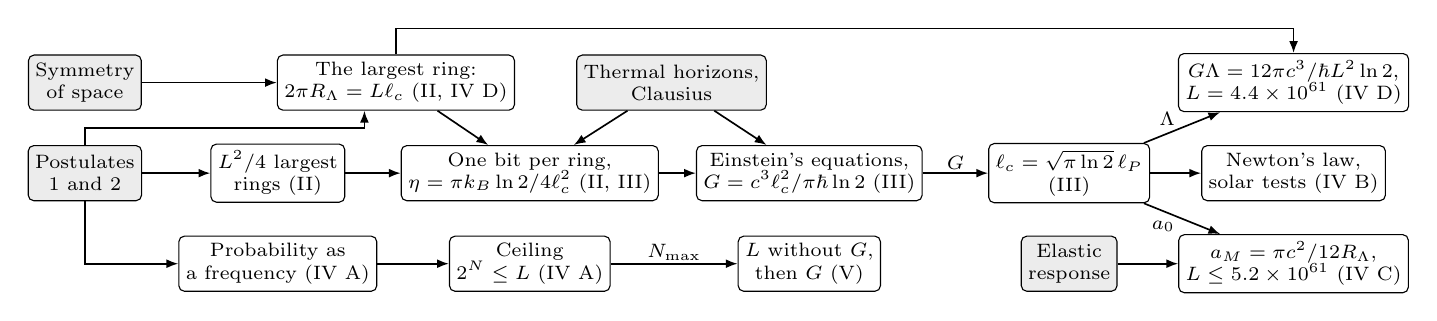
\begin{tikzpicture}[x=1cm,y=1cm,
  inp/.style={draw, fill=gray!15, rounded corners=2pt, align=center, font=\scriptsize, inner sep=2.5pt, minimum height=7mm},
  res/.style={draw, rounded corners=2pt, align=center, font=\scriptsize, inner sep=2.5pt, minimum height=7mm},
  arr/.style={-{Latex[length=1.5mm]}, semithick},
  lab/.style={font=\scriptsize, inner sep=1pt}]
\node[inp] (P)  at (0.80,0)   {Postulates\\1 and 2};
\node[res] (C)  at (3.25,0)   {$L^2/4$ largest\\rings (II)};
\node[res] (E)  at (6.45,0)   {One bit per ring,\\$\eta = \pi k_B\ln2/4\lc^2$ (II, III)};
\node[res] (EQ) at (10.0,0)   {Einstein's equations,\\$G = c^3\lc^2/\pi\hbar\ln2$ (III)};
\node[res] (LC) at (13.30,0)  {$\lc = \sqrt{\pi\ln2}\,\ell_P$\\(III)};
\node[res] (NW) at (16.15,0)  {Newton's law,\\solar tests (IV B)};
\node[res] (PL) at (4.75,1.15) {The largest ring:\\$2\pi\RL = L\lc$ (II, IV D)};
\node[inp] (TH) at (8.25,1.15) {Thermal horizons,\\Clausius};
\node[inp] (SY) at (0.80,1.15) {Symmetry\\of space};
\node[res] (GL) at (16.15,1.15) {$G\Lambda = 12\pi c^3/\hbar L^2\ln2$,\\$L = 4.4\times10^{61}$ (IV D)};
\node[res] (PR) at (3.25,-1.15) {Probability as\\a frequency (IV A)};
\node[res] (CE) at (6.45,-1.15) {Ceiling\\$2^N\le L$ (IV A)};
\node[res] (LQ) at (10.0,-1.15) {$L$ without $G$,\\then $G$ (V)};
\node[inp] (EL) at (13.30,-1.15) {Elastic\\response};
\node[res] (AM) at (16.15,-1.15) {$a_M = \pi c^2/12\RL$,\\$L\le5.2\times10^{61}$ (IV C)};
\draw[arr] (P) -- (C); \draw[arr] (C) -- (E);
\draw[arr] (SY) -- (PL);
\draw[arr] (P.north) -- ++(0,0.22) -| ([xshift=-4mm]PL.south);
\draw[arr] (PL) -- (E);
\draw[arr] (TH) -- (E); \draw[arr] (E) -- (EQ);
\draw[arr] (TH) -- (EQ);
\draw[arr] (EQ) -- node[lab, above]{$G$} (LC); \draw[arr] (LC) -- (NW);
\draw[arr] (LC) -- node[lab, above left, pos=0.45]{$\Lambda$} (GL);
\draw[arr] (PL.north) -- ++(0,0.33) -| (GL.north);
\draw[arr] (LC) -- node[lab, below left, pos=0.45]{$a_0$} (AM);
\draw[arr] (EL) -- (AM); \draw[arr] (P.south) |- (PR.west);
\draw[arr] (PR) -- (CE); \draw[arr] (CE) -- node[lab, above]{$N_{\max}$} (LQ);
\end{tikzpicture}
\caption{The derivation. Shaded boxes are inputs, labels on arrows are measured values, and no arrow runs back; the readings of the postulates (Sec.~\ref{sec:count}) are steps of the text and are not boxed; the radius of the largest ring enters twice, in a ring's share of area and, once Sec.~\ref{sec:cosmo} shows it is the horizon's, in $\Lambda = 3/\RL^2$.}
\label{fig:tree}
\end{figure*}

\section{Postulates and Count}
\label{sec:postulates}

Two postulates define the register. A \emph{ring} is a closed line of translation in space; a \emph{cell} is a place on a ring; a \emph{tick} is the time light takes to cross a cell; a \emph{largest ring} is a ring of $L$ cells, the most a ring has (Postulate~1); a \emph{qubit} is a two-level quantum system, whatever realizes it.

\textbf{Postulate 1 (the register).} \emph{Quantum mechanics is granular. Every qubit is a string of bits, one on each cell of a ring, each cell of length $\lc$, which light crosses in one tick. No ring has more than $L$ cells, with $L\in\mathbb{N}$. The bits are the possible outcomes of one measurement of the qubit, and the string's cyclic position on its ring is the qubit's phase. Any two qubits can be measured jointly. The shift moves every bit of a string one cell along its ring per tick. The global phase of a state is hidden: no law depends on it.}

\textbf{Postulate 2 (the rings).} \emph{Every cell has one opposite, the cell halfway around every largest ring through it. Any two cells not opposite lie on one largest ring, any two largest rings share a cell, and no ring holds every cell.}

We read Postulate~1 as putting one string on each ring, with a bit on each of the ring's cells; a cell that lies on several rings holds a bit of each. We do not assume the length of a cell, $\lc$: Sec.~\ref{sec:count} derives $G$ in terms of it, and the measured $G$ then fixes it at $\sqrt{\pi\ln2}$ Planck lengths. The cell's tick, energy, mass, and acceleration are then $\tc = \lc/c$, $\Ec = \hbar c/\lc$, $\mc = \hbar/c\lc$, and $\ac = c^2/\lc$, and a mass $M$ is $\alpha = M/\mc$ cell masses. The shift carries a string once around a largest ring in $L$ ticks, its lap time $L\tc$.

\textbf{The horizon's area.} A largest ring is a closed line of $L$ cells of length $\lc$, a closed geodesic of length $L\lc$. Let $\RL$ be the radius of a circle of that length,
\begin{equation}
\RL = \frac{L\,\lc}{2\pi} ;
\label{eq:ident}
\end{equation}
Sec.~\ref{sec:cosmo} derives from Einstein's equations, solved without a mass, that each largest ring is such a circle and that every observer at rest has a cosmological horizon, a sphere of the same radius, of area $A_{\rm hor} = 4\pi\RL^2 = L^2\lc^2/\pi$. What that derivation uses is the form of the equations, not the entropy density that this area fixes in Sec.~\ref{sec:count}, on which the solution without a mass does not depend. In the glossary above, space is what the shift moves a string through, cell by cell along its ring. The manifold, the smooth space of lengths and areas in which Sec.~\ref{sec:cosmo} reads a ring as a closed geodesic and a horizon as a sphere, describes it at that scale. Rest and acceleration are the manifold's descriptions of a body; the register does not define them, since in it every string moves one cell per tick (Postulate~1). In the manifold, an observer or a body at rest is unaccelerated, and the geometry about it does not change in time. The horizon counted here is that of an observer at rest in the solution without a mass, the state the universe approaches (Sec.~\ref{sec:cosmo}); the horizons of different observers differ in place, not in radius or count, since Postulate~2 distinguishes no cell. What the manifold does not describe is the register's incidence, which rings share a cell: the count below makes the register a finite projective plane, which cannot be drawn with its points on a sphere and its lines as great circles, by the Sylvester--Gallai theorem~\cite{erdos1943}, and the postulates do not ask that it be. What the count and the horizon share is a number, $R$ rings for the area $A_{\rm hor}$, each ring worth $A_{\rm hor}/R$ of it. That identification is a reading, the first of five the paper makes (Sec.~\ref{sec:count}), and it is all the horizon's geometry contributes: the count never uses the places of cells. Everything physical is in the register: by Postulate~1 a body is strings of bits on rings, so it occupies some cells, and its rings are largest rings of the register, each a great circle of the horizon of some observer at rest (Sec.~\ref{sec:cosmo}).

\textbf{The count.} Postulate~2 fixes the number of cells and rings, and this count is the new input to gravity. An opposite lies halfway around a ring of $L$ cells, so $L$ is even. Every largest ring through a cell $P$ passes through its opposite $P'$, and two rings through $P$ share only $P$ and $P'$, since two cells not opposite fix one ring. So the rings through $P$ cut the remaining cells into disjoint sets of $L-2$. Any two largest rings share a cell (Postulate~2), and with it its opposite. Take a largest ring $A$ through $P$, which exists since $P$ and any cell not opposite it lie on one (Postulate~2), and a cell $Q$ off it (Postulate~2). With $S$ a cell of $A$ other than $P$ and $P'$, the cells $Q$ and $S$ are not opposite, since the opposite of $S$ lies on $A$, so one largest ring $E$ passes through both. It misses $P$, since the one ring through $P$ and $S$ is $A$, which does not hold $Q$. Each ring through $P$ meets $E$ in one opposite pair, distinct rings in distinct pairs, and every pair of $E$ lies on a ring through $P$; $E$ has $L/2$ pairs, so $\rho = L/2$ rings pass through every cell. Every cell not opposite $P$ lies on one of them, so the register has
\begin{equation}
\begin{split}
C &= 2 + \rho(L-2) = \frac{L^2}{2} - L + 2 \ \text{cells},\\
R &= \frac{C\rho}{L} = \frac{L^2}{4} - \frac{L}{2} + 1 \ \text{rings},
\end{split}
\label{eq:counts}
\end{equation}
and $C = 2R$: one ring for every opposite pair of cells. With a cell and its opposite taken as a point and a largest ring as a line, the register is a finite projective plane of order $L/2 - 1$ (for $L\ge6$), with $R$ points and $R$ lines. That constrains $L$: every known plane has prime-power order, and Bruck and Ryser exclude many others~\cite{bruck1949}. To leading order in $1/L$, a ring's share of the sphere's area is $A_{\rm hor}/R = 4\lc^2/\pi$.

\textbf{The entropy.} A horizon's entropy counts what can change in the strings that describe it. Every ring carries one string, which moves along its ring as a whole, one cell per tick (Postulate~1), in one of the ring's two senses; what can change in a free string is which way it moves, a doublet, and the sense it moves in is what a measurement returns, the bit of the cell read (Postulate~1). Interactions, which emit, absorb, create, or annihilate particles, add and remove strings~\cite{korytko2026d}. Between interactions all the mass and light of the universe is strings moving one way or the other along their rings, and the count is of that. What interactions add is a correction, small for matter that stays put rather than radiating itself away; every mass of the sections below is such matter. A string's energy is set by its motion and is the same either way along its ring, since nothing in the postulates prefers a sense of a ring, so the horizon's thermal state (Sec.~\ref{sec:count}) weights the two senses equally, and a doublet weighted equally holds one bit, $k_B\ln2$, the most a qubit can hold. The string's bits are the possible outcomes of measuring that doublet (Postulate~1): a bit marked $1$ is the outcome in which the string moves one way, a bit marked $-1$ the other~\cite{korytko2026c}, so its fraction of 1s is the probability of moving one way and its position on the ring the phase between the two amplitudes, and together they are the state of that one qubit, Eq.~(\ref{eq:raqm}). The $L$ positions are the values its phase can take, not further states: a string is one qubit, its Hilbert space is two-dimensional, and its entropy is at most that one bit. So a horizon's entropy is one bit for each ring of the register, the count identified with its area (above): the horizon of an observer at rest holds
\begin{equation}
\frac{S_{\rm hor}}{k_B} = R\ln2 = \frac{L^2}{4}\ln2
\label{eq:S}
\end{equation}
to leading order. It comes from the register's count, not from Bekenstein and Hawking; Sec.~\ref{sec:count} shows that, with the cell fixed by the measured $G$, it equals their quarter per Planck area.

\textbf{Counting in the bulk.} The count is exact for the horizon of the solution without a mass (above). One premise enters here from outside the postulates, the symmetry of space: a largest ring can run through a cell in any direction, and no direction is preferred. A sphere of radius $r$ about a body holds the strings that cross its surface, and its entropy is one bit for each, the direction of its motion, as on a horizon. The register does not count them: it fixes how many cells lie at each distance from the body, $L$ (Sec.~\ref{sec:galactic}), and with them a sphere's incidences, $L^2/2$ at every distance, $L/2$ rings through each of its cells, but not which rings those are, since a ring not through the body meets each ring through it once, at a distance the postulates leave free. Averaged over those distances, as Sec.~\ref{sec:galactic} averages, every ring has two cells on every sphere: the incidence of the register knows no distance, and counted by it every sphere would hold all $L^2/4$ strings. The number of a sphere's strings is read instead from its area, one string for each ring's share of it: Postulate~2 distinguishes no cell and the symmetry of space no direction, so that share, $4\lc^2/\pi$, is the same everywhere. This is the area law of a screen, a closed surface whose entropy is read from its area as a horizon's is~\cite{verlinde2011,padmanabhan2010}, the one reading taken beyond the cosmological horizon; Sec.~\ref{sec:count} uses it on every local horizon, and Sec.~\ref{sec:galactic} is where it carries weight. The sphere holds the fraction $(r/\RL)^2$ of the largest rings, its area in units of a ring's share: with $n = r/\lc$ the distance in cells,
\begin{equation}
N_s(r) = \frac{L^2}{4}\Big(\frac{r}{\RL}\Big)^2 = \pi^2 n^2
\label{eq:N}
\end{equation}
strings. These are shares of area, not places: at each distance from a body there are $L$ cells, two on each of its rings (Sec.~\ref{sec:galactic}). $L$ cancels between the horizon's count and the unit, so the strings of a sphere at solar radii go as $n^2$, with $n^2\ll L^2$, and do not involve $L$. Areas, light cones, and the Raychaudhuri equation are written as in Jacobson's argument (Sec.~\ref{sec:count}); the register constructs no manifold, and what it adds is the count.

\textbf{The reversal.} We keep Palmer's picture of state reduction as a shift map, one step per tick by Postulate~1, so that $\tau^* = L\tc$, but with $L$ universal. The shift is the free evolution itself. The companion paper~\cite{korytko2026c} reads a string's pattern as a wave, and a wave with $\kappa$ wavelengths around the ring gains $\kappa$ steps of phase per tick, $e^{-iEt/\hbar}$ with $E = \kappa hc/L\lc$, so the energy $h/\tau^*$ that goes with a single step per tick is that of the lowest mode, $\kappa = 1$, the lap of the largest ring, and not every qubit's; nothing here uses that reading, since here a string's arrangement carries no meaning (Sec.~\ref{sec:quantum}) and the shift is only the clock. With $L$ a constant of nature the map cannot lower it; the reversal keeps only its clock, $L$ ticks. Then, by Eq.~(\ref{eq:ident}),
\begin{equation}
\tau^* = L\,\tc = \frac{2\pi\RL}{c} ,
\label{eq:clock}
\end{equation}
the lap time of a largest ring, $2\pi/H_\infty$ with $H_\infty = c/\RL$. The universal energy that replaces $E_G$ is then
\begin{equation}
\frac{\Ec}{L} = \frac{\hbar}{\tau^*} = \frac{\hbar c}{2\pi\RL} = k_B T_{\rm dS},
\label{eq:energy}
\end{equation}
the Gibbons--Hawking temperature of a horizon of radius $\RL$~\cite{gibbons1977}. Palmer's Eq.~(\ref{eq:palmerL}), read backwards, says that gravity's characteristic energy in the reduction process is the thermal energy of the cosmological horizon, and that every qubit shares it. Three consequences follow at once. First, $\tau^*\sim10^{11}$~yr, so an isolated qubit never completes reduction; Palmer makes the same observation. Second, $L$ no longer depends on the qubit, so $N_{\max}$ is the same for every technology, which is the sharpest experimental difference between the two causal orderings. Third, the reversal discards mass-dependent gravitational collapse, which Palmer's program takes to be gravity's role in quantum mechanics~\cite{palmer2016}. In Palmer's ordering a heavy superposition has small $L$ and reduces in milliseconds; here every system shares the same clock, so the definiteness of macroscopic bodies is not supplied by gravity and must come, as in standard quantum theory, from environmental decoherence. The reversed theory therefore predicts no mass-dependent collapse signal of Di\'osi--Penrose type; the null result of the underground search of Ref.~\cite{donadi2021} is consistent with it and, since Palmer's shift map is non-dissipative, with his ordering too, so it does not discriminate.

\section{Newton's Constant from the Count}
\label{sec:count}

Before testing the hypothesis at widely separated scales, we derive $G$ from the count of Sec.~\ref{sec:postulates} and the thermodynamics of horizons. In all, the paper takes from outside the postulates the symmetry of space (Sec.~\ref{sec:postulates}), the two thermodynamic inputs of this section, Verlinde's elastic response (Sec.~\ref{sec:galactic}), and the first law of thermodynamics for the cosmic fluid (Sec.~\ref{sec:predictions}), none of them a number. It reads the postulates in five places. The count is identified with the horizon's area, a ring's share being $4\lc^2/\pi$ (Sec.~\ref{sec:postulates}); each ring carries one string (Sec.~\ref{sec:postulates}); a screen obeys the area law, one bit per ring's share of area on every horizon and on a sphere that is not one (Secs.~\ref{sec:postulates} and \ref{sec:count}); a string's bit is spread evenly over its cells inside the horizon (Sec.~\ref{sec:galactic}); and a joint measurement reads its strings in step, the $k$-th bit of each together (Sec.~\ref{sec:quantum}). Of general relativity it takes as known the Schwarzschild--de~Sitter solution, the surface gravity of its horizons, and the closed geodesics of de Sitter space (Sec.~\ref{sec:cosmo}), Komar's energy with Padmanabhan's equipartition (Sec.~\ref{sec:cell}), the Deser--Levin temperature (Sec.~\ref{sec:galactic}), and the perihelion and deflection formulas (Sec.~\ref{sec:solar}).

Here two things enter. A horizon is thermal: its state is periodic in imaginary time, and a state with imaginary-time period $\tau$ has temperature $k_BT = \hbar/\tau$, which is the Kubo--Martin--Schwinger condition~\cite{kubo1957}. The period of a horizon is $2\pi c/a$, with $a$ its surface gravity, which is the content of the Unruh and Gibbons--Hawking temperatures~\cite{unruh1976,gibbons1977}; for a horizon of radius $\RL$ it is the lap time of a largest ring, Eq.~(\ref{eq:clock}). The energy that crosses a horizon is heat, $\delta Q = T\,dS$, which is Jacobson's step~\cite{jacobson1995}. He assumes that the entropy per unit area is the same on every horizon; here the entropy comes from the register, Eq.~(\ref{eq:S}), which fixes that density, and since a ring's share of area is the same everywhere (Sec.~\ref{sec:postulates}), the density is the same on every horizon. This is where the count adds to Jacobson's derivation, in which the density is a free parameter fixed by Newton's constant: here it is the same parameter, and it stays fixed by $G$ through the cell until $L$ is measured (Sec.~\ref{sec:hold}), but the largest ring ties it to $\Lambda$ (Sec.~\ref{sec:cosmo}) and the ceiling to $L$. We do not use Verlinde's entropic argument for Newton's law~\cite{verlinde2011}, whose force driven by a screen's entropy is the contested step~\cite{visser2011}; Jacobson's argument has no force, and the elastic response of Verlinde's later work~\cite{verlinde2017}, a different argument, enters in Sec.~\ref{sec:galactic}.

\subsection{The temperature of a horizon in cells}
In cells, a horizon whose period is $L_h$ ticks, $\tau = L_h\tc$, has by the thermal assumption the temperature
\begin{equation}
k_B T = \frac{\hbar}{L_h\tc} = \frac{\Ec}{L_h} .
\label{eq:T}
\end{equation}
For the horizon of radius $\RL$ the period is the lap time of a largest ring, $L_h = L$, and Eq.~(\ref{eq:T}) is Eq.~(\ref{eq:energy}). An observer accelerating at $a$ has a horizon $c^2/a$ behind him, whose period is $2\pi c/a$, that is, $L_a = 2\pi c^2/a\lc$ ticks; Eq.~(\ref{eq:T}) then gives $k_BT_a = \hbar a/2\pi c$, Unruh's temperature. Through every point of spacetime, in every null direction, passes the horizon of such an observer, a local Rindler horizon.

\subsection{Clausius relation}
On every local Rindler horizon the entropy is one bit per ring's share of area, the area law of Sec.~\ref{sec:postulates}, so Jacobson's balance of heat and entropy reads
\begin{equation}
\delta Q = T_a\,dS = k_BT_a\ln2\,dR = \frac{\hbar a\ln2}{2\pi c}\,dR :
\label{eq:clausius}
\end{equation}
each ring a horizon gains takes in $k_BT_a\ln2$, its temperature times one bit of entropy, which is Landauer's energy of a bit~\cite{landauer1961}. Energy crossing a horizon therefore adds rings, $2\pi c/(\hbar a\ln2)$ of them per unit of energy, and with a ring's share of area $4\lc^2/\pi$ it adds area $dA = [8\lc^2 c/(\hbar a\ln2)]\,\delta Q$. The Raychaudhuri equation gives the change of area in terms of the Ricci tensor, and the balance can hold in every direction at every point only if
\begin{equation}
R_{\mu\nu} - \tfrac12 R\,g_{\mu\nu} + \Lambda g_{\mu\nu} = \frac{2\pi k_B}{\hbar c\,\eta}\,T_{\mu\nu},
\label{eq:einstein}
\end{equation}
with $\eta$ the entropy per unit area and $\Lambda$ an integration constant that the argument leaves free. A stress tensor proportional to the metric has no flux through a null surface, so it never enters Eq.~(\ref{eq:clausius})~\cite{jacobson1995,korytko2026b}. This is Einstein's equation, and comparing its coefficient with $8\pi G/c^4$ gives $G = c^3k_B/4\hbar\eta$. Nothing in this is a force: Eq.~(\ref{eq:einstein}) is a condition on the geometry, that the count of every local horizon stays in balance with the heat that crosses it, and matter then moves on the geodesics of the geometry that satisfies it.

\subsection{The cell from Newton's constant}\label{sec:cell}
By Eqs.~(\ref{eq:counts}) and (\ref{eq:S}) the entropy per unit area of the horizon is, to leading order in $1/L$, $\eta = k_B R\ln2/A_{\rm hor} = k_B(L^2/4)\ln2/(L^2\lc^2/\pi)$, so
\begin{equation}
\eta = \frac{\pi k_B\ln2}{4\lc^2}, \qquad
G = \frac{c^3\lc^2}{\pi\hbar\ln2} = \frac{4\pi c^3\RL^2}{\hbar L^2\ln2} .
\label{eq:G}
\end{equation}
This is the result of the section. The $\pi$ comes from a ring's share of area, $4\lc^2/\pi$, and the $\ln2$ from the bit; Jacobson's $4$, from the $8\pi$ of the field equations and the $2\pi$ of the thermal period, cancels the $4$ of that share. Newton's constant is measured, so Eq.~(\ref{eq:G}) fixes the cell,
\begin{equation}
\lc = \sqrt{\frac{\pi\ln2\,\hbar G}{c^3}} = \sqrt{\pi\ln2}\,\ell_P = 2.39\times10^{-35}~{\rm m},
\label{eq:cell}
\end{equation}
with $\ell_P \equiv \sqrt{\hbar G/c^3} = \lc/\sqrt{\pi\ln2}$,
so the Planck length is a derived quantity, the cell over $\sqrt{\pi\ln2}$. With it the horizon's entropy, Eq.~(\ref{eq:S}), is $S_{\rm hor}/k_B = (L^2/4)\ln2 = \pi^2\RL^2\ln2/\lc^2 = \pi\RL^2/\ell_P^2 = A_{\rm hor}/4\ell_P^2$: Bekenstein and Hawking's quarter per Planck area~\cite{bekenstein1973} is the register's one bit per ring, a ring's share of the horizon being $4\ell_P^2\ln2$. The quarter itself follows from Jacobson's coefficient and the measured $G$ for any count; the count fixes the cell. Newton's law, $a = GM/r^2$, is the weak-field limit of Eq.~(\ref{eq:einstein}). Its content for a static sphere is Padmanabhan's equipartition~\cite{padmanabhan2010}, which holds in every static solution of Eq.~(\ref{eq:einstein}). The Komar energy inside a sphere on which the acceleration is $a$, the energy that gravitates, is twice its entropy times the temperature, $Mc^2 = 2T_aS$~\cite{komar1959}, two Landauer energies $k_BT_a\ln2$ for each of its strings,
\begin{equation}
\begin{split}
Mc^2 &= 2N_s(r)\,k_BT_a\ln2 = \pi n^2\ln2\,\frac{\hbar a}{c}\\
&\Longrightarrow\quad \frac{a}{\ac} = \frac{\alpha}{\pi n^2\ln2} ,
\end{split}
\label{eq:newton}
\end{equation}
with $\alpha$ and $n$ as in Sec.~\ref{sec:postulates}. So Newton's law reads: the body's energy is shared equally by the strings of any sphere around it; the share per string is set by the temperature of the horizon that an observer held on the sphere sees; and the share falls as $1/r^2$, since the number of strings grows as $r^2$. Two remarks follow. First, what the count adds. Where Jacobson leaves $\eta$ free, here it is a count, one bit per ring's share of area, $\pi k_B\ln2/4\lc^2$, so the measured $G$ fixes the cell and, through the largest ring, ties $G$ to $L$ and to $\Lambda$ (Sec.~\ref{sec:cosmo}), and the same $L$ caps a quantum computer (Sec.~\ref{sec:quantum}); where Verlinde postulates the volume law and its coefficient, here the law follows from the area law of a screen and the count of a string's share inside a sphere, and the coefficient is his, normalized where the solution puts the horizon, a quarter lap along a ring (Sec.~\ref{sec:galactic}). Without cells there is no count, and $\eta$ stays free. Second, Eq.~(\ref{eq:G}) scales as $1/L^2$: with $L$ a constant of nature, $G$ is constant exactly when the horizon radius is; this singles out the de Sitter horizon (Sec.~\ref{sec:cosmo}) and makes the constancy of $G$ and of $\Lambda$ one statement (Sec.~\ref{sec:predictions}).

\section{Gravitational Phenomena Scale by Scale}
\label{sec:scales}

On each scale one structure of the register does the work, and we record what each scale pins. At the solar scale it is the sphere of Eq.~(\ref{eq:N}); at the galactic scale the string, a largest ring whose cells run from the sphere out to the horizon, $L/4$ cells from the body; at the cosmological scale the closed ring.

\subsection{Quantum scale: qubits and quantum computers}\label{sec:quantum}

Probabilities need no further postulate. A measurement returns the bit of one cell (Postulate~1), so the probability of the outcome $1$ is the sum over the cells of the probability that a cell is read times its bit. Whatever law picks the cell can use only the state, and Postulate~1 gives a string's bits meaning as outcomes and its position as phase, and nothing else: the arrangement of the bits, which cells carry the 1s, is no part of the state. So no law picks a cell by its bit, since that needs the arrangement; the probability that a cell is read depends on the state and the cell alone, and the probability of an outcome must be the same for every arrangement that has the same state. In a string with both kinds of bit, exchanging a $1$ and a $-1$ between two cells must then leave it unchanged, which, with the reading probabilities fixed, holds only if the two cells are read with the same probability; for strings measured jointly, whose bits are paired position by position (below), the exchange is of two positions in all of them at once, which keeps every pairing and with it the joint state. So every cell is read alike, and every probability is a frequency over the ring's bits: Eq.~(\ref{eq:raqm}) holds, with the ring's length for $L$. This is not the principle of indifference: a law that read a fixed offset from the string's position, say, is excluded because it would return the bit that the reference arrangement, a convention, puts there.

On this scale $L$ acts directly, through Eq.~(\ref{eq:nmax}), and the joint measurement of Postulate~1 shows which states it limits. Qubits measured jointly are read together bit by bit, one bit of each string at a time, so that every bit of a later string comes paired with one outcome of the earlier qubits. This is how we read \emph{measured jointly}: a joint measurement is one measurement, and its possible outcomes are the bits of the strings measured, paired position by position, the $k$-th bit of each string forming the $k$-th possible outcome. The reading is the fifth the paper makes (Sec.~\ref{sec:count}), and it is Palmer's, whose state of $N$ qubits is $N$ correlated strings of $L$ bits with one permutation applied to all of them~\cite{palmer2026}; it does not require the strings to share a cell, and it is all that the count below uses. The cells of a later string whose bits are paired with one joint outcome of the earlier qubits form a \emph{block} of the string, and blocks of different outcomes are disjoint. The fraction of 1s on a block is the probability of the outcome 1 given the block's joint outcome, and the probability of a joint outcome is the product, string by string, of the frequencies of its bits on its blocks. A block whose fraction lies strictly between 0 and 1 needs at least two cells, one reading 1 and one reading 0. In a random state, each of the $2^{N-1}$ joint outcomes of the first $N-1$ qubits occurs, and given it the last qubit's bit is 1 with probability strictly between 0 and 1. Its string then needs $2^{N-1}$ blocks of at least two cells, so $2^N$ is at most its length, and $2^N\le L$. A qubit's string is a largest ring of the register, of $L$ cells, so the ceiling is $\lfloor\log_2L\rfloor = 204$, at $204.8$ (Sec.~\ref{sec:hold}); a string on a shorter ring, which Postulate~1 allows, only lowers it, and $2^N\le L$ holds in every case. The shortening of a horizon's throat by a mass inside it (Sec.~\ref{sec:galactic}) does not touch the register's rings. The bound is not the random state's alone. It holds for every state in which all $2^N$ joint outcomes occur, since each of them takes at least one of the $L$ positions, and a product state of $N$ qubits, each in a superposition, is such a state: its last string needs the same $2^{N-1}$ blocks of two cells. A state of the Greenberger--Horne--Zeilinger type escapes it, with two joint outcomes and blocks of fraction 0 or 1, one cell each. Most product states are not held exactly even at small $N$: two qubits prepared apart, with the fractions $m_1/L$ and $m_2/L$, have the joint frequency $m_1m_2/L^2$ for the outcome $(1,1)$, a multiple of $1/L$ only when $L$ divides $m_1m_2$. Postulate~1 fixes each string exactly, its fraction and position, and the pairing only up to its $L$ positions; such a state is held with its strings exact and its pairing approximate, and which pairing the postulates do not say. That latitude does not soften the bound, which is on the pairing itself: no pairing of $L$ positions holds more than $L$ joint outcomes. What singles out the random state is that only there do the missing outcomes show, as the test below explains.

Random-circuit sampling up to $83$ qubits~\cite{gao2025} is consistent with $2^{83}\le L$, though at cross-entropy fidelities below 1\% it does not establish it, and 83 is in any case far below $\log_2L = 204.8$, so this scale does not yet pin $L$. A count of physical qubits, far larger, is not a count of qubits in a random state, and the bound shows nothing in it, for the reason given below. Logical qubits count as physical ones do: a logical qubit is a two-level system, so Postulate~1 gives it a string of its own (Sec.~\ref{sec:postulates}), whatever the strings of the physical qubits that realize it, and the $48$ demonstrated on $280$ atoms~\cite{bluvstein2024} lie far below the ceiling. On the timescale Palmer gives for factoring tests~\cite{palmer2026}, this scale will measure $L$ directly. The test is a random circuit on $N$ fault-tolerant logical qubits, deep enough to produce a random state, followed by its inverse. In quantum mechanics the state returns to the initial one with the gate fidelity; here it does not once $N$ exceeds $\log_2L$. The intermediate state cannot be the random state, since at least $2^N - L$ of its joint outcomes are missing, a fraction $1 - L/2^N$ of them: 15\% at $N = 205$ and more than half at $206$ (Appendix~\ref{app:numbers}). The inverse circuit acts on the pairing through its gates on pairs of qubits, and it returns the initial state only from the pairing it was built to undo. A product state at the same $N$, as the register holds it, lacks joint outcomes too. But it is prepared and undone by gates on single qubits, each of which changes one qubit's state, its string's fraction and position (Postulate~1), which are exact at every $N$; so every qubit returns. Nor does measuring it show anything, since no sample shows which of $2^N$ outcomes are missing. That is why the random circuit tests the bound and a product state does not. By how much the random state fails to return is not derived here, nor how well it returns just below $\log_2L$, where the blocks are a few cells wide (Sec.~\ref{sec:hold}): the postulates fix the capacity, not which state a circuit produces when it calls for more blocks than a string has room for. Error correction does not lift the ceiling, which is set by room and not by errors. The reversed theory's prediction on this scale is a ceiling of $204$, tested one way: a return at $205$ or more falsifies it (Sec.~\ref{sec:predictions}).

\subsection{Terrestrial and solar scales: the sphere}\label{sec:solar}

Section~\ref{sec:count} gave Einstein's equations with $G = c^3\lc^2/(\pi\hbar\ln2)$, Eq.~(\ref{eq:G}), and Newton's law as their weak-field limit, Eq.~(\ref{eq:newton}). Gravitational redshift, the perihelion advance of Mercury, light deflection, and gravitational-wave propagation then follow as they do in general relativity. Mercury's anomalous advance $6\pi GM_\odot/(p\,c^2)$, with $p = a_{\rm orb}(1-e^2)$ the semi-latus rectum of the orbit, is $42.98''$ per century and the deflection of starlight at the solar limb $4GM_\odot/(c^2R_\odot)$ is $1.75''$, both as observed. At the Earth's orbit, $\alpha = 1.35\times10^{38}$ and $n = 6.27\times10^{45}$ in Eq.~(\ref{eq:newton}) give $5.93\times10^{-3}$~m\,s$^{-2}$. They depend on $L$ and $\RL$ only through $G$, i.e., only through the cell $\lc = 2\pi\RL/L$.

This scale therefore pins $\lc$, the combination $2\pi\RL/L$, and not $L$ on its own. The count of a sphere is $n^2$, with $L$ cancelled against the unit, Eq.~(\ref{eq:N}); and the horizon of an observer held at solar radii is his own, $L_a\ll L$, since $a\gg c^2/\RL$ there. This is as it should be, since solar-system gravity is described by general relativity to exquisite precision, and a theory in which $L$ showed up there separately from $\RL$ would be wrong. The horizon could enter solar-system dynamics by two routes. The push of Sec.~\ref{sec:cosmo} reaches the planets, but with only $5\times10^{-25}$~m\,s$^{-2}$ at the Earth's orbit. For an isolated Sun the elastic response of Sec.~\ref{sec:galactic} stops short of them: a sphere about the Sun is saturated, and Newton's law holds exactly, out to the crossing of Eq.~(\ref{eq:criterion}), where $GM_\odot/r^2 = c^2/\pi\RL$, $5900$~au from the Sun. The Sun is not isolated, though: in modified-Poisson versions of MOND the Galaxy's field adds a quadrupole to the Sun's, which Cassini's ranging bounds at $Q_2 = (3\pm3)\times10^{-27}$~s$^{-2}$, excluding the standard transitions~\cite{hees2014}. The counts above are for an isolated mass, the framework has as yet no field equation for a second one, and that bound is what a treatment of two masses would have to meet.

\subsection{Galactic scale: the string}\label{sec:galactic}

At the scales above, $L$ and $\RL$ entered gravity only through their ratio, and two facts of the register played no part. The strings of a sphere have $L$ bits, one on each cell of a largest ring, and reach the horizon. And no ring has more than $L$ cells, and no horizon is colder than $\Ec/L$: in de Sitter space an observer held at acceleration $a$ sees the two horizons combined in quadrature, $k_BT = (\hbar/2\pi c)\sqrt{a^2 + a_\Lambda^2}$ with $a_\Lambda = c^2/\RL$~\cite{deser1997}, never below $\Ec/L$, whatever $a$ is. The floor is on the temperature, not on the acceleration. Both facts enter at accelerations of order the horizon's surface gravity, $c^2/\RL = cH_\infty = 5.4\times10^{-10}$~m\,s$^{-2}$. That the scale at which rotation curves flatten is the horizon's acceleration, up to a coefficient, is not ours: Milgrom reached it from the Unruh temperature of de Sitter space~\cite{milgrom1999}, and Verlinde from its entanglement entropy~\cite{verlinde2017}. Ours is the share of a string inside a sphere, counted in cells along its ring to the horizon, which the solution puts a quarter lap away: it fixes where $L$ enters, and it makes the coefficient Verlinde's, normalized at the quarter lap. We derive it by following his elastic argument with that share in place of his normalization of the volume law.

\textit{A mass draws the horizon in.} Einstein's equations were derived in Sec.~\ref{sec:count}. Their solution for a mass $M$ at rest inside the cosmological horizon, treated as a point with $GM/c^2\ll\RL$, is Schwarzschild--de Sitter~\cite{kottler1918}, whose outer horizon lies at $\RL - GM/c^2$ to first order in $M$. By Eq.~(\ref{eq:cell}), $GM/c^2 = \lc\alpha/(\pi\ln2)$: the mass draws the horizon in by $\alpha/(\pi\ln2)$ cells. Its circumference is $L_M = L - 2\alpha/\ln2$ cells, and the area law (Sec.~\ref{sec:postulates}), one bit per ring's share of area, gives it $L_M^2/4$ bits, the number Eq.~(\ref{eq:counts}) would give with $L_M$ in place of $L$; the closed geodesics at its throat, of $L_M$ cells, are the shorter rings Postulate~1 allows (Sec.~\ref{sec:cosmo}). The horizon's entropy is then $(\ln2)/4$ times the square of its circumference in cells, Eq.~(\ref{eq:S}) with $L_M$ for $L$, and the loss is $(L/2)\cdot(2\alpha/\ln2)\cdot\ln2$,
\begin{equation}
S_M = L\alpha = \frac{Mc^2}{k_BT_{\rm dS}} = \frac{2\pi Mc\RL}{\hbar} ,
\label{eq:SM}
\end{equation}
which is Verlinde's result, Eq.~(25) of Ref.~\cite{verlinde2017} (SciPost numbering here and below), in cells. The entropy a mass takes from the horizon is its mass in cell masses times the length of the ring in cells, or its energy over the horizon's temperature, and it does not depend on the cell's size. Within a sphere of radius $r\ll\RL$ the mass removes entropy the same way. A sphere's area grows with geodesic distance at $8\pi$ times its radius less $8\pi GM/c^2$, so out to $r$, far outside the body, it falls short by $8\pi GMr/c^2$. At a ring's share $4\lc^2/\pi$ that is $2\pi n\alpha/\ln2$ rings, one bit each, so the mass removes $S_M(r) = 2\pi n\alpha = 2\pi Mcr/\hbar$. At $r = \RL$ this is Eq.~(\ref{eq:SM}), and it agrees with Verlinde's Eq.~(28).

\textit{Where the strings hold their entropy.} The body occupies some cells of largest rings of the register (Sec.~\ref{sec:postulates}), and we draw a sphere of radius $r$ about it that encloses it, with $r$ far larger than the body's size. Distances are counted from the cell at the center of that sphere, which treats the body as a point, as Newton's law does. Postulate~2 gives every other cell a distance from the center: the number of steps between them, the shorter way round, along the one largest ring through both. One cell is an exception: the cell opposite the center lies on every one of the $L/2$ rings through the center, always $L/2$ steps away, so its distance is $L/2$ by any of them. Between the two, each of those rings holds two cells at every distance, one each way round, so every distance from $1$ to $L/2 - 1$ has $L$ cells. The horizon of a body at rest lies $L/4$ cells out, at the proper distance $\pi\RL/2 = L\lc/4$ that Sec.~\ref{sec:cosmo} derives, a quarter of a largest ring, to leading order in $M$; inside it are the cells nearer to the center than to the cell opposite it. The sphere of radius $r$, whose cells lie at distance $n = r/\lc$ from the center, holds $N_s(r) = \pi^2n^2$ strings, Eq.~(\ref{eq:N}), read from its area (Sec.~\ref{sec:postulates}), not counted from its cells, which number $L$. Its strings are not confined to it: each lies on a largest ring through a cell of the sphere, and the ring runs on to the horizon. Along a ring the distance is proper distance, since each cell has length $\lc$ (Postulate~1) and a ring is a closed geodesic (Sec.~\ref{sec:cosmo}); it equals the areal radius of Eq.~(\ref{eq:N}), the $r$ for which the sphere's area is $4\pi r^2$, when $r\ll\RL$, the only case used below, and at the horizon the two are $L/4$ and $L/2\pi$ cells. The two cells of an opposite pair lie at the distances $d$ and $L/2 - d$, one on each side of the horizon or both on it, and every largest ring is made of $L/2$ such pairs, since it passes through the opposite of each of its cells. So every string has half its cells, $L/2$ of them, inside the horizon or on it, counting a cell on it as half. Its entropy, one bit, is which way it moves, and the body's observer, who never sees beyond his horizon (Sec.~\ref{sec:cosmo}), describes a string by its half inside, which holds the whole bit. The bit is which way the string moves, a property of the whole string and not of a cell, so where along the half it sits is not fixed by the postulates. The count uses only the average over the many strings through a sphere, and over them no cell is preferred (Sec.~\ref{sec:quantum}), so on average the bit is spread evenly over the $L/2$ cells, the fourth reading of Sec.~\ref{sec:count}.

The largest rings through a cell $P$ of the sphere, apart from the one through the body, hold between them every cell off that ring exactly once. Such a cell is not opposite $P$, so one largest ring passes through both, and it is not the ring through the body. Besides $P$ and its opposite, which lie on all of them, these rings hold $L-2$ cells at each distance from $1$ to $L/2-1$, and the ring through the body holds two. So the rings through $P$ spread their cells inside the horizon evenly over the distances up to $L/4$, and $n$ of every $L/4$ lie inside the sphere. To leading order in $1/n$, the entropy the sphere's strings hold inside it is therefore the fraction $n/(L/4) = 4n/L$ of their $N_s(r)$ bits,
\begin{equation}
S_{\rm in}(r) = \frac{4n}{L}\,N_s(r)\ln2 = \frac{4\pi^2 n^3}{L}\ln2 ,
\label{eq:volume}
\end{equation}
a volume law. Verlinde postulates a volume law for the entanglement entropy of de Sitter space, the horizon entropy divided evenly over the bulk, and normalizes it on a flat ball of radius $\RL$, which gives the fraction $2\pi n/L$; his Eq.~(81) makes each cell's contribution the ratio of its proper distance from the center to the horizon's. Here the law follows from the area law of a screen, the reading that gives the strings of the sphere, and one count, the share of a string inside it by its cells, where its bit is: the horizon is at $\pi\RL/2$ along a ring, not at $\RL$, and that is the whole difference between our $\pi/12$ and his $1/6$. The share is not the length of the ring inside the sphere, which would depend on the angle at which the ring meets it; that would place the string's cells in the manifold, which the register does not do (Sec.~\ref{sec:postulates}). While the mass removes more entropy within the sphere than its strings hold there, $S_M(r) > S_{\rm in}(r)$, the sphere is saturated: what fixes the share is the two-dimensional count of Eq.~(\ref{eq:N}), and Newton's law holds. The crossing is where the two are equal,
\begin{equation}
S_M(r) = S_{\rm in}(r): \quad N_s = \frac{\pi L\alpha}{2\ln2}, \quad g_N = \frac{c^2}{\pi\RL} ,
\label{eq:criterion}
\end{equation}
so rotation curves depart from Newton's law at an acceleration of order the horizon's.

\textit{The elastic response.} Below the crossing the entropy inside the sphere exceeds what the mass removes, and the remainder responds as an incompressible elastic medium. The removed entropy occupies the volume $V_M = S_M(r)\,V_0$, with $V_0 = V(r)/S_{\rm in}(r) = L\lc^3/(3\pi\ln2)$ the volume per unit of entropy from Eq.~(\ref{eq:volume}). The strain $\varepsilon$ outside the removed region obeys $\int_0^r \varepsilon^2 A\,dr' \le V_M(r)$, with equality under Verlinde's assumption on the principal strain (his Sec.~7.1, Eqs.~(44)--(46) and (88)): the largest principal strain takes the greatest value the removed entropy allows, and the strains perpendicular to it are equal. The strain gives the apparent surface mass density, $\Sigma_D = (a_\Lambda/8\pi G)\,\varepsilon$ with $a_\Lambda = c^2/\RL$, his Eq.~(43). The energy of a strain is quadratic in it, so the apparent mass goes as the square root of the removed entropy. With equality, differentiating at fixed $M$ gives $\varepsilon^2 = (1/A)\,dV_M/dr$, and with Gauss's law $\Sigma = g/4\pi G$,
\begin{equation}
g_D^2 = a_M\,g_N, \quad a_M = \frac{\pi}{12}\,\frac{c^2}{\RL} = 1.42\times10^{-10}~{\rm m\,s^{-2}} ,
\label{eq:aM}
\end{equation}
which is $(\pi^2/6)\,c^2/L\lc$. Without equality, Eq.~(\ref{eq:aM}) is an upper bound in the deep regime, the distances at which $g_D$ far exceeds $g_N$. There the apparent mass $M_D$, the mass whose Newtonian field is $g_D$, grows as $r$, so $\varepsilon^2A$, which goes as $(M_D/r)^2$, tends to a constant. The mean of $\varepsilon^2A$ out to $r$, which the inequality keeps below $V_M/r = dV_M/dr$, tends to the same constant, and so the constant is at most $dV_M/dr$. With equality, $M_D = M\,n\sqrt{\pi^3\ln2/6L\alpha}$: it grows by a fixed amount per cell of distance, as the part of a string inside the sphere does. The total field is $g = g_N + g_D$, and in the deep regime
\begin{equation}
g = \sqrt{a_M\,g_N},\qquad v_c^4 = a_M\,G\,M ,
\label{eq:btfr}
\end{equation}
flat rotation curves and the baryonic Tully--Fisher relation, with $M$ the baryonic mass alone. This is Milgrom's phenomenology~\cite{milgrom1983}, which the radial acceleration relation confirms as a tight empirical law across galaxy types~\cite{mcgaugh2016}. That one $a_0$ serves galaxies whose stellar masses span five orders of magnitude is explained here only if the bound is saturated; the bound alone does not explain it. The measured scale is $a_0 = (1.20\pm0.02\pm0.24)\times10^{-10}$~m\,s$^{-2}$~\cite{mcgaugh2016}, and $(1.19\pm0.04\pm0.09)\times10^{-10}$ when each galaxy's distance, inclination and mass-to-light ratios are fitted along with it~\cite{desmond2023}. Both lie below Eq.~(\ref{eq:aM}), as the bound requires, at 85\% and 84\% of it; the test is one-sided, and it is passed. Whether the bound is saturated, as it is under Verlinde's assumption on the principal strain, is a second question: the first measurement leaves it open, at $0.9\sigma$ below the bound, and the second puts it in doubt, at $2.3\sigma$ below. With Verlinde's coefficient the observed $a_0$ would exceed the bound. For attribution, the coefficients in units of $cH_\infty$ are: $1$, Milgrom's vacuum scale~\cite{milgrom1999}; $1/6 = 0.17$, Verlinde's Eq.~(102)~\cite{verlinde2017}, which gives $0.90\times10^{-10}$~m\,s$^{-2}$ with our $\RL$; $\pi/12 = 0.26$, this paper, $\pi/2$ larger than his; against $0.22$ observed. Verlinde's specific interpolation between the Newtonian and deep regimes shows tension with the radial acceleration relation in the transition region~\cite{lelli2017}; what pins $L$ here is the deep-regime scaling (\ref{eq:btfr}), which survives that test, and the transition function remains open.

\textit{Why the temperature cannot lead.} The floor $\Ec/L$ could be taken as the mechanism instead of the bits. If gravity followed the excess of the combined temperature over the floor, as Milgrom proposed~\cite{milgrom1999}, Eq.~(\ref{eq:newton}) would give $a = \sqrt{g_N^2 + 2a_\Lambda g_N}$. That has the right deep form, with $a_M = 2c^2/\RL$, nine times the observed value, and a transition 38\% above Newton's law at $g_N = 10a_0$, where the observed relation is 4\% above. The floor marks the scale; the law is in the strings.

To be explicit: in this framework there is no dark-matter halo, nor the smearing of energy-momentum over neighboring space-times by which Invariant Set Theory reaches the same phenomena with $\Lambda = 0$~\cite{palmer2016,hance2025}. Galactic rotation is set by the baryons, $G$, and the horizon radius, which $\Lambda$ fixes. The known difficulties of any such account, galaxy clusters~\cite{clowe2006} and the acoustic peaks of the microwave background~\cite{planck2018}, are not addressed here and remain open.

This scale bounds $L$. The deep-regime law is observed, and weak lensing now extends it to circular velocities that stay flat out to a megaparsec, on the same baryonic Tully--Fisher relation~\cite{mistele2024}. Setting Eq.~(\ref{eq:aM}) equal to the measured $a_0$,
\begin{equation}
L_{\rm gal} = \frac{\pi^2}{6}\,\frac{c^2}{a_0\,\lc} = 5.2\times10^{61}.
\label{eq:Lgal}
\end{equation}
Since Eq.~(\ref{eq:aM}) is a bound, so is this: $L \le 5.2\times10^{61}$, with equality where the bound is saturated.

\subsection{Cosmological scale: the ring}
\label{sec:cosmo}

Einstein's equations, Eq.~(\ref{eq:einstein}), leave $\Lambda$ free. Without a mass, and with the symmetry of space (Sec.~\ref{sec:postulates}), their solution has maximally symmetric spatial sections, and the vacuum solutions with $\Lambda$ and such sections are the maximally symmetric spacetime for the sign of $\Lambda$: flat space, de Sitter space, or anti-de Sitter space~\cite{hawking1973}. A ring is a closed line of translation, a closed geodesic of space, and of the three only de Sitter space has one: flat and anti-de Sitter space have no closed spacelike geodesic. De Sitter space is the hyperboloid $-v^2 + w^2 + x^2 + y^2 + z^2 = 3/\Lambda$ in five-dimensional Minkowski space, and its closed geodesics are its sections by the spacelike two-planes through the origin: circles of radius $\sqrt{3/\Lambda}$, all of one length, each a great circle of the cosmological horizon of some observer at rest~\cite{hawking1973}. So $\Lambda > 0$, and every ring has the length $2\pi\sqrt{3/\Lambda}$, each a great circle of the horizon of some observer at rest; for a largest ring, of length $L\lc$, Eq.~(\ref{eq:ident}) gives $\sqrt{3/\Lambda} = \RL$, so $\Lambda = 3/\RL^2$, which fixes the integration constant.

In de Sitter space an observer at rest has a cosmological horizon, the farthest he can ever see, of radius $\sqrt{3/\Lambda} = \RL$ and at the proper distance $\pi\RL/2$ from him, a quarter lap of a largest ring~\cite{gibbons1977}. In the register his horizon is the $L$ cells a quarter lap from his cell, $L/4$ steps along each ring through it, and what he sees is the cells nearer to his than to the cell opposite it. Every largest ring, through his cell or not, has half its cells there or on the horizon, since its cells come in opposite pairs at the distances $d$ and $L/2 - d$ from his cell (Sec.~\ref{sec:galactic}). That half carries the entropy inside his horizon; the horizon's own entropy is the register's count identified with its area, Eq.~(\ref{eq:S}). The manifold puts him at the center of a two-sphere of area $4\pi\RL^2$ that holds $L^2/4$ strings by the area law, each of its great circles a closed geodesic of a ring's length; the paper uses only what the two agree on, the number of strings, one bit each, the area per string, and the quarter lap. Which closed geodesics the rings are, neither says: any two rings share a cell, which two great circles of a three-sphere need not, so the register's incidence is not the manifold's (Sec.~\ref{sec:postulates}).

The horizon's period is $2\pi\RL/c$, the lap time of a largest ring, which is the content of Eq.~(\ref{eq:energy}). With Eq.~(\ref{eq:G}), Newton's constant and the cosmological constant are then not independent of each other,
\begin{equation}
G\,\Lambda = \frac{12\pi c^3}{\hbar\,L^2\ln2}.
\label{eq:Lambda}
\end{equation}
The strength of gravity and the acceleration of the universe are tied into one constant, with $L$ as the exchange rate between them. The observed $\Lambda = 1.09\times10^{-52}$~m$^{-2}$~\cite{planck2018} gives the horizon radius $\RL = \sqrt{3/\Lambda} = 1.66\times10^{26}$~m, and Eq.~(\ref{eq:ident}) with the cell of Eq.~(\ref{eq:cell}) gives
\begin{equation}
L_{\rm cos} = \frac{2\pi\RL}{\lc} = 4.4\times10^{61}.
\label{eq:Lcos}
\end{equation}
Only two measurements enter, $\Lambda$ and, through the cell, $G$.

The argument has come full circle, so it is worth saying in what order it runs. Section~\ref{sec:postulates} counted the largest rings and gave every observer's horizon one bit for each; no solution of any equation was used. Section~\ref{sec:count} derived Einstein's equations from that count. Their solution without a mass has closed geodesics of one length, a largest ring's, so the count left no ring out; had it allowed shorter ones, they would have carried bits the count did not include, and the equations would not describe the space they produce. That they do is a check on the count, not one of its premises. The solution with a mass, Schwarzschild--de~Sitter, has closed geodesics at the throats of its horizons, where $f = 0$ and the sphere of constant $r$ is totally geodesic in the static slice: the great circles of the cosmological horizon, of $L_M = L - 2\alpha/\ln2$ cells (Sec.~\ref{sec:galactic}), and, for a black hole, of its own horizon, of $L' = 4\pi GM/c^2\lc$ cells. These are the shorter rings Postulate~1 allows, outside the count of Postulate~2, and they are where a mass is counted: by the area law a horizon with a mass $M$ inside holds $L_M^2/4$ bits (Sec.~\ref{sec:galactic}), and a black hole's horizon holds $(L'^2/4)\ln2 = \pi r_s^2/\ell_P^2$, which is $A/4\ell_P^2$. The register's rings stay the largest rings: a body's cells lie on them, they cross its horizon with half their cells inside and carry the entropy inside it (Sec.~\ref{sec:galactic}), and $2^N\le L$ holds for every string (Sec.~\ref{sec:quantum}). The actual universe, with its matter, is not the massless solution either, nor is its matter a mass at rest inside a horizon, the case of Eq.~(\ref{eq:SM}): it is neither at rest nor a point mass. Even counted as one it would be too heavy for the solution. At today's mean density of matter, the fraction $\Omega_m = 0.315$ of the critical density $3H_0^2/8\pi G$, a ball of radius $\RL$ holds a mass with $GM/c^2 = (\Omega_m/2\Omega_\Lambda)\RL = 0.23\RL$, beyond the limit $\RL/3\sqrt3 = 0.19\RL$ up to which the Schwarzschild--de~Sitter solution has a horizon at all (Appendix~\ref{app:numbers}). So nothing is claimed here for the entropy of the horizon today. The horizon of radius $\RL$ is that of the de Sitter state the universe approaches, at the rate $H_\infty = H_0\sqrt{\Omega_\Lambda}$ (Appendix~\ref{app:numbers}), and it is that horizon that Sec.~\ref{sec:postulates} counts. The one thing the solution adds is its integration constant, $\Lambda = 3/\RL^2$, which the equations leave free and the count never assumed.

The structure at this scale is the closed ring: $L$ cells, a fixed number, and no ring of the register is larger. An observer's horizon holds one bit for each of the $L^2/4$ of them, Eq.~(\ref{eq:S}), at the temperature $\Ec/L$, Eq.~(\ref{eq:energy}), so its energy, entropy times temperature, is one Landauer energy for each string,
\begin{equation}
E_\Lambda = \frac{L^2}{4}\,\frac{\Ec}{L}\ln2 = \frac{L\,\Ec}{4}\ln2 = \frac{c^4\RL}{2G} = 1.0\times10^{70}~{\rm J},
\label{eq:EL}
\end{equation}
and the last equality uses Eq.~(\ref{eq:G}). Spread over the interior, the flat ball of areal radius $\RL$ in which the Misner--Sharp relation below is exact, it is $\rho_\Lambda = 3\pi^2\rho_c\ln2/2L^2 = 5.3\times10^{-10}$~J\,m$^{-3}$, with $\rho_c = \Ec/\lc^3$; the areal radius measures area and the ring measures distance, so the density uses $\RL$ and the share of Sec.~\ref{sec:galactic} the quarter lap, each where it is exact. One factor of $L$ comes from counting a sphere rather than a volume, and one from a string's energy, $(\Ec/L)\ln2$; this is how Ref.~\cite{korytko2026b} closes the $123$ orders of magnitude of the vacuum energy. The energy of Eq.~(\ref{eq:EL}) is that of a constant density with pressure $-\rho_\Lambda$, which is the same as saying it has no flux through null surfaces; it is the Misner--Sharp energy of the horizon~\cite{misner1964}, the density times the volume, one Landauer energy per string. The energy that gravitates is the Komar energy of Eq.~(\ref{eq:newton}), which counts the pressure three times, $\rho + 3p = -2\rho_\Lambda$: it is $-2E_\Lambda$, two Landauer energies per string as for a mass, but negative. In the weak field about a mass $M$ the solution of Eq.~(\ref{eq:einstein}) is Schwarzschild--de Sitter, and its acceleration toward the mass is
\begin{equation}
g(r) = \frac{GM}{r^2} - \frac{c^2 r}{\RL^2}, \qquad \frac{a}{\ac} = \frac{\alpha}{\pi n^2\ln2} - \frac{4\pi^2 n}{L^2} .
\label{eq:push}
\end{equation}
The second term is the push: the horizon's surface gravity scaled by $r/\RL$. Every free body recedes from every other, which is de Sitter expansion at $H_\infty = c/\RL = 2\pi/L\tc$, the Hubble rate being $2\pi$ over the lap time of Eq.~(\ref{eq:clock}). Against the Newtonian pull the push would balance at $r_z^3 = GM\RL^2/c^2$, where each equals $c^2r_z/\RL^2$. That is below the crossing value $c^2/\pi\RL$ of Eq.~(\ref{eq:criterion}) whenever $r_z < \RL/\pi$, which holds for any galaxy, group or cluster, so the pull that meets the push is that of Eq.~(\ref{eq:btfr}). The two balance at $r = \RL v_c/c$, in cells $n = Lv_c/2\pi c$, which is $3.7$~Mpc for an isolated mass of $10^{11}M_\odot$; no galaxy is isolated at that distance, but the order holds: flat rotation curves end where the ring's push overtakes the string's pull, beyond the megaparsec to which weak lensing now finds them flat~\cite{mistele2024}.

The horizon is the de Sitter one, constant in time, and observation requires that: $L$ is a constant, so by Eqs.~(\ref{eq:ident}) and (\ref{eq:G}) the cell and $G$ scale with the radius. Were the horizon the Hubble radius $R_H = c/H$ with $L$ fixed, then $G\propto R_H^2$ would drift at $\dot G/G = 2H(1+q)\approx6\times10^{-11}$~yr$^{-1}$, with $q\approx-0.53$ the present deceleration parameter, six hundred times the lunar-laser-ranging bound~\cite{hofmann2018}. With $\RL$ constant, $G$, $a_M$ and $\Lambda$ are all constant, as Eq.~(\ref{eq:Lambda}) requires, and since every observer's de Sitter horizon has the same radius, $L$ is observer-independent, as a constant of nature must be.

\section{Does $L$ Hold?}
\label{sec:hold}

Table~\ref{tab:pins} collects the results. Two scales bear on $L$, each with the cell from the measured $G$: one gives a bound, the other a value. The galactic scale, through the acceleration at which rotation curves flatten and the coefficient of Eq.~(\ref{eq:aM}), gives $L \le 5.2\times10^{61}$. The cosmological scale, through the size of the de Sitter horizon, gives $4.4\times10^{61}$, which lies inside the bound, at 85\% of it, a quarter of a bit below in $\log_2L$: $204.8$ against $205.0$, so the value gives $N_{\max} = 204$ and the bound, if saturated, $205$, by less than a hundredth of a bit. The two come from scales five orders of magnitude apart, and their consistency does not test the power of ten, which both take from the cell; $\lc$ cancels in the ratio $L_{\rm gal}/L_{\rm cos} = \pi c^2/12 a_0\RL$. It tests the coefficient: that $c^2/a_0$ is at least $12\RL/\pi$, as Sec.~\ref{sec:galactic} gives.

The scale is not new: it is the coincidence $a_0\sim cH_0$ that Milgrom noted in 1983~\cite{milgrom1983} and has since written as $2\pi a_0\approx cH_0\approx c^2\sqrt{\Lambda/3}$, leaving open which of the two $a_0$ is tied to~\cite{milgrom2020}. The framework adds four things. It fixes the coefficient, as an upper bound that observation respects. It ties $a_0$ to $\RL$ rather than to $H(z)$, so the scale does not evolve. It turns the coincidence into a fixed relation, $\Lambda = 432\,a_M^2/\pi^2c^4$, from Eq.~(\ref{eq:aM}) and $\Lambda = 3/\RL^2$. And it ties the same $L$ to a third quantity that has nothing to do with either galaxies or cosmology: the number of qubits a quantum computer can bring into a random state. That third pin measures $L$ on its own, without $G$, and it is still to come.

\begin{table*}[t]
\caption{What each scale derives from $L$ and $\RL$, what it imports from outside the postulates, and what it pins. The symmetry of space (Sec.~\ref{sec:postulates}) enters every scale but the quantum one. Since $\lc = 2\pi\RL/L$, pinning $\lc$ pins only the ratio of $\RL$ to $L$. The chain is run with $G$ as input and $\lc$ as output until $N_{\max}$ is measured.}
\label{tab:pins}
\begin{ruledtabular}
\small\setlength{\tabcolsep}{4pt}
\begin{tabular}{lllll}
Scale & Phenomenon & Relation & Imports & Pins \\
\colrule
Quantum & qubit ceiling & $N_{\max}=\lfloor\log_2L\rfloor$ & none & $L$ (to come) \\
Earth & Newton's law & $G=c^3\lc^2/(\pi\hbar\ln2)$ & thermal horizon; Clausius & $\lc$ \\
Solar & GR tests & same $G$ & as above & $\lc$ \\
Galactic & rotation curves & $a_M=\pi c^2/12\RL$ & elastic response; RAR data & $L\le5.2\!\times\!10^{61}$ \\
Cosmic & horizon radius & $\lc=2\pi\RL/L$ & measured $\Lambda$ & $L=4.4\!\times\!10^{61}$ \\
\end{tabular}
\end{ruledtabular}
\end{table*}

The quantum scale will pin $L$ directly. The bound $2^N\le L$ gives $N_{\max}=204$ at the value of $L$ from $\Lambda$ (Appendix~\ref{app:numbers}). The ceiling is sharp on one side only. At $205$ or more no string has room for a block of two cells for every joint outcome, so no random state can be held there. Below it the bound is soft, and by more than a unit. A block of $r$ cells resolves the last qubit's conditional probability to one part in $r$, so a random state whose conditional probabilities are resolved that finely needs $2^{N-1}r\le L$, that is $N\le\log_2(2L/r)$: $202$ for one part in $10$, $200$ for one part in $30$, and $199$ for one part in $100$ (Appendix~\ref{app:numbers}). At $204$ itself the blocks average $L/2^{203} = 3.4$ cells, so a random state is held there only coarsely, its conditional probabilities rounded to the few values that blocks of three or four cells allow. The expected signature is therefore a loss of return that grows over the last few qubits below $204$, not a wall at it; by how much is not derived (Sec.~\ref{sec:quantum}), and the test is one-sided, a return with the gate fidelity at $205$ or more falsifying. Palmer's bit count $2^{N+1}-2\le NL$, which gives $211$~\cite{palmer2026c}, is the weaker condition. It charges one bit for each real parameter of the state, but bits do not run out: a string whose $L$ blocks hold one cell each uses all its bits, yet every fraction on it is 0 or 1. What runs out is room, two cells for each block (Sec.~\ref{sec:quantum}). Neither touches the point that matters: the ceiling is universal. Palmer's per-qubit values of $L$ would put it at $212$ for a quantum-dot electron and $362$ for a hyperfine ion-trap qubit (he rounds $10^{109}$ to $2^{400}$ and writes $N_{\max}\approx400$~\cite{palmer2026}); ceilings that differ with the technology would restore his causal order; the same value for all confirms ours.

That measurement also runs the derivation the other way, as the title promises. With $L$ known, Eq.~(\ref{eq:ident}) gives the cell from the size of the universe, and Eq.~(\ref{eq:G}) gives Newton's constant. Gravity's strength is then a derived quantity: the number of rings of the register, one bit each on an observer's horizon. A measured ceiling $N_{\rm obs}$ is at most $\lfloor\log_2 L\rfloor$, so it gives a lower bound on $L$, $2^{N_{\rm obs}}\le L$, and with Eq.~(\ref{eq:G}) an upper bound on $G$; if the ceiling is where the bound itself is reached, $2^{N_{\rm obs}}\le L<2^{N_{\rm obs}+1}$, $L$ follows to a factor of two, $\lc$ to a factor of two, and $G$ to a factor of four. A ceiling of $204$ then brackets $G$ between $4.8\times10^{-11}$ and $1.9\times10^{-10}$~m$^3$\,kg$^{-1}$\,s$^{-2}$, and the measured value lies inside the bracket, at $\log_2 L = 204.8$. Only the quantum computer separates $L$ from $\lc$.

The universal $L$ found here lies below every per-qubit value Palmer obtains from Eq.~(\ref{eq:palmerL}), so if both mechanisms were at work, the cosmological one would bind. And Davies' bound~\cite{davies2007}, which Palmer flagged as suspiciously close to his own numbers, is the horizon's count: an observer's horizon holds $L^2/4 = 4.8\times10^{122}$ bits, the $10^{122}$ Davies takes for the universe, and the $N\approx400$ Palmer quotes for it ($\log_210^{122} = 405$) is its logarithm, $2\log_2L - 2 = 407.5$, to the precision of the estimate; the capacity bound counts the string length $L$, not the bits of the horizon, so $N_{\max} = \log_2L\approx204$, half his exponent.

\section{Predictions and Falsification}
\label{sec:predictions}

\begin{enumerate}
\item \textbf{A universal ceiling of at most 204 qubits} in a random state, the same for photonic, trapped-ion, superconducting and semiconductor qubits, insensitive to isolation and to logical error correction. The test is the random circuit and its inverse of Sec.~\ref{sec:quantum}. A return with the gate fidelity at $205$ or more logical qubits falsifies the ceiling; technology dependence of a ceiling falsifies the reversal and restores Eq.~(\ref{eq:palmerL}).
\item {\boldmath\textbf{Newton's constant from the ceiling.}} $G = 4\pi c^3\RL^2/(\hbar L^2\ln2)$, Eq.~(\ref{eq:G}), with $2^N\le L$ for every $N$ at which a random state returns: a measured ceiling bounds $G$ from above, and if it is where the bound is reached it gives $G$ to a factor of four. The same return at $205$ or more logical qubits falsifies Eq.~(\ref{eq:G}); a lower ceiling does not, since how the return degrades below the bound is not derived (Sec.~\ref{sec:quantum}).
\item \textbf{Rotation curves from baryons alone}, flat in the deep regime under Verlinde's equality on the strain, with $v_c^4 = a_M G M_{\rm baryon}$, Eq.~(\ref{eq:btfr}), and in any case bounded: $a_M = \pi c^2/12\RL = 1.4\times10^{-10}$~m\,s$^{-2}$, Eq.~(\ref{eq:aM}), is an upper bound on the acceleration scale of the flat regime. A measured $a_0$ above $1.4\times10^{-10}$~m\,s$^{-2}$, robust detection of a dark-matter particle, or a galaxy whose rotation curve requires dark matter, falsifies the galactic sector. That loses the second pin of $L$; the horizon pin, Eq.~(\ref{eq:Lcos}), the relation~(\ref{eq:Lambda}), and items~1 and~2 do not use it.
\item {\boldmath\textbf{No redshift evolution of $a_0$.}} The acceleration scale is tied to the constant $\RL$ of the horizon, not to $H(z)$; proposals with $a_0\propto cH(z)$ predict a scale $1.8$ times larger at redshift $z=1$, and this framework predicts no change.
\item {\boldmath\textbf{Constancy of $\Lambda$.}} With $L$ fixed, Eq.~(\ref{eq:G}) gives $G\propto\RL^2$ at one bit per ring, a string's entropy when matter stays put (Sec.~\ref{sec:postulates}), so the lunar-laser-ranging bound on $\dot G/G$~\cite{hofmann2018} requires the horizon radius, and with it $\Lambda$, to be constant to one part in $10^{13}$ per year, and their product $G\Lambda = 12\pi c^3/(\hbar L^2\ln2)$, Eq.~(\ref{eq:Lambda}), is fixed by $L$ alone. Since a dark-energy component with equation of state $w$ evolves as $\dot\rho/\rho = -3H(1+w)$, and the expansion rate carries $\Lambda$ as the term $\Lambda c^2/3$, this is, within the framework, a bound on the present-day equation of state, $|1+w_0| \lesssim 5\times10^{-4}$ (Appendix~\ref{app:numbers}). It applies to the present epoch, the only one lunar laser ranging probes. DESI DR2 prefers evolving dark energy over a constant $\Lambda$ at $2.7\sigma$ in one analysis~\cite{desi2026} and at up to $4.2\sigma$ in another, depending on the probes combined~\cite{desi2025}. A confirmed evolution is incompatible with the framework as stated: here $w=-1$ is not assumed, as in $\Lambda$CDM, but follows from $L$ and $\lc$ being constant, so the framework predicts that the preference will not survive.
\end{enumerate}

\section{Conclusion}

Palmer built a discrete quantum mechanics and used gravity to set its granularity. We have argued that the granularity comes first. Two postulates about cells and rings, with the thermodynamics of horizons, fix the number of rings of the register and make an observer's horizon's entropy one bit per ring; through Jacobson's argument they give general relativity with Newton's constant in terms of the cell, so that the Planck length is the cell over $\sqrt{\pi\ln2}$ and Bekenstein and Hawking's quarter per Planck area is one bit per ring, and they bind Newton's constant and the cosmological constant into one. With Verlinde's elastic response added, they bound from above the acceleration scale of flat rotation curves without dark matter, with his coefficient normalized where the solution puts the horizon. Read backwards, Palmer's collapse formula gives a universal reduction clock, the de Sitter period, and mass-dependent gravitational collapse drops out. The two scales that fix $L$ in gravity, each with the measured $G$, are consistent: the value from the horizon lies inside the galactic bound, and since the cell cancels between them, what that tests is the coefficient of the galactic scale. The measurement of $L$ on its own is a quantum computer's, and the ceiling is testable within the decade.

\begin{acknowledgments}
The author used Anthropic's Claude as a research assistant. Under the author's direction it checked the literature, recomputed the numbers, wrote the Lean formalization, and edited text. The author checked every edit, including Lean code, inputs, and results. The physical proposal, the postulates, and the claims are the author's own.
\end{acknowledgments}

\par\medskip\centerline{\small\bfseries DECLARATIONS}\par\smallskip
\noindent\textbf{Funding.} No funding was received for this work.\\
\textbf{Competing interests.} The author declares no competing interests.\\
\textbf{Data availability.} No new data were generated. All numerical inputs are published values cited in the text and tabulated in Appendix~\ref{app:numbers}. A Lean~4 formalization, RegisterGravity v13, is deposited with this preprint and at \url{https://github.com/AlphaLatitude/RegisterGravity/tree/v13}, archived by Software Heritage as \swhid{swh:1:rel:9141c2e50d65530a58c677131f8a4ba982eab37e;origin=https://github.com/AlphaLatitude/RegisterGravity;visit=swh:1:snp:79b434bf8598792e3f3f74e39414bb8ecd76e1ea}. It checks the count of Sec.~\ref{sec:postulates}, each relation of the paper from the count with every input of Sec.~\ref{sec:count} a named hypothesis (Jacobson's argument enters as the coefficient of Einstein's equations), and every number of Appendix~\ref{app:numbers}. The five readings of the postulates (Sec.~\ref{sec:count}) enter the files as named definitions, the pairing of a joint measurement as the function that gives, at each cell of a string, the outcome the other qubits show. Of the classical results of Einstein's equations, the Schwarzschild--de~Sitter solution~\cite{kottler1918}, the surface gravity of its horizons, the closed geodesics of de Sitter space, that the spheres of constant $r$ at the horizons of Schwarzschild--de~Sitter space are totally geodesic, and the perihelion and deflection formulas are taken as known.\\
\textbf{Preprint.} A preprint of this manuscript was first deposited at Zenodo on 2 September 2026, \url{https://doi.org/10.5281/zenodo.22255462}.\\
\textbf{Use of AI tools.} As stated in the Acknowledgments; the author takes full responsibility for the manuscript.

\appendix

\section{Numerical Values}
\label{app:numbers}

Inputs. $c = 2.998\times10^8$~m\,s$^{-1}$, $\hbar = 1.055\times10^{-34}$~J\,s, $G = 6.674\times10^{-11}$~m$^3$\,kg$^{-1}$\,s$^{-2}$ (the Lean files use the CODATA values $299\,792\,458$, $1.054\,571\,817\times10^{-34}$ and $6.674\,30\times10^{-11}$, and for the Sun the IAU heliocentric constant below), hence $\ell_P = 1.616\times10^{-35}$~m and, by Eq.~(\ref{eq:cell}), the cell $\lc = \sqrt{\pi\ln2}\,\ell_P = 2.385\times10^{-35}$~m, $\tc = \lc/c = 7.96\times10^{-44}$~s, $\mc = \hbar/c\lc = 1.475\times10^{-8}$~kg, $\Ec = \hbar c/\lc = 1.326\times10^9$~J, $\ac = c^2/\lc = 3.77\times10^{51}$~m\,s$^{-2}$; $a_0 = 1.20\times10^{-10}$~m\,s$^{-2}$~\cite{mcgaugh2016}; present Hubble rate $H_0 = 67.4$~km\,s$^{-1}$\,Mpc$^{-1}$, dark-energy density parameter $\Omega_\Lambda = 0.685$ and matter density parameter $\Omega_m = 0.315$~\cite{planck2018}, giving $H_\infty = H_0\sqrt{\Omega_\Lambda} = 1.81\times10^{-18}$~s$^{-1}$, $\Lambda = 3H_\infty^2/c^2 = 1.09\times10^{-52}$~m$^{-2}$, $\RL = c/H_\infty = 1.66\times10^{26}$~m; lunar laser ranging $\dot G/G = (7.1\pm7.6)\times10^{-14}$~yr$^{-1}$~\cite{hofmann2018}, taken as $|\dot G/G|\lesssim10^{-13}$~yr$^{-1}$.

Derived. $L_{\rm cos} = 2\pi\RL/\lc = 4.37\times10^{61}$, $\log_2 = 204.76$. $a_M = \pi c^2/12\RL = 1.42\times10^{-10}$~m\,s$^{-2}$, and $L_{\rm gal} = (\pi^2/6)c^2/(a_0\lc) = 5.17\times10^{61}$, $\log_2 = 205.01$. Ratio $1.18$. Capacity condition $2^N\le L$: $2^{204} = 2.57\times10^{61}\le L_{\rm cos} < 2^{205} = 5.14\times10^{61}$, so $N_{\max}=204$, with $2^{204}$ and $2^{205}$ at $0.59$ and $1.18$ of $L_{\rm cos}$; $L_{\rm gal}$ lies just above $2^{205}$. Planck's uncertainties in $H_0$ and $\Omega_\Lambda$ move $\log_2L_{\rm cos}$ by about $\pm0.02$, and the local $H_0 = 73$~km\,s$^{-1}$\,Mpc$^{-1}$ would give $204.65$; the ceiling is $204$ either way. Blocks of $r$ cells, $2^{N-1}r\le L_{\rm cos}$: $N_{\max} = 202$, $200$ and $199$ for $r = 10$, $30$ and $100$; at $N = 204$ the blocks average $L_{\rm cos}/2^{203} = 3.4$ cells; at $N = 205$ and $206$ the missing joint outcomes are the fraction $1 - L_{\rm cos}/2^N = 0.15$ and $0.58$. The Galaxy, $M = 10^{12}M_\odot = 2.0\times10^{42}$~kg, a mass at rest, has $\alpha = 1.35\times10^{50}$ and $2\alpha/\ln2 = 3.9\times10^{50}$, one part in $10^{11}$ of $L_{\rm cos}$; the matter of a ball of radius $\RL$ at today's mean density, $\Omega_m\cdot3H_0^2/8\pi G$, is not such a mass (Sec.~\ref{sec:cosmo}): its $GM/c^2\RL = \Omega_m/2\Omega_\Lambda = 0.23$ exceeds the limit $1/3\sqrt3 = 0.19$ up to which the Schwarzschild--de~Sitter solution has a horizon (the Nariai limit). Reduction clock $\tau^* = L_{\rm cos}\tc = 3.5\times10^{18}$~s $= 1.1\times10^{11}$~yr. Energy $\Ec/L_{\rm cos} = 3.03\times10^{-53}$~J $= \hbar H_\infty/2\pi$. Register: $L^2/2 = 9.5\times10^{122}$ cells and $L^2/4 = 4.8\times10^{122}$ rings; an observer's horizon holds $(L^2/4)\ln2 = 3.3\times10^{122}$, equal to $\pi\RL^2/\ell_P^2$. Equation~(\ref{eq:G}) with $L = 2^{204}$ and $2^{205}$ brackets $G$ between $1.93\times10^{-10}$ and $4.82\times10^{-11}$~m$^3$\,kg$^{-1}$\,s$^{-2}$; with $L_{\rm cos}$ it returns the input, $6.67\times10^{-11}$. Sun, with $M_\odot = GM_\odot/G$ from the heliocentric constant $GM_\odot = 1.327\times10^{20}$~m$^3$\,s$^{-2}$: $\alpha = M_\odot/\mc = 1.35\times10^{38}$, $GM_\odot/c^2\lc = \alpha/(\pi\ln2) = 6.19\times10^{37}$ cells, $L\alpha = 5.9\times10^{99}$; Earth's orbit $n = 6.27\times10^{45}$, $\ac\alpha/(\pi n^2\ln2) = 5.93\times10^{-3}$~m\,s$^{-2}$. $E_\Lambda = (L\Ec/4)\ln2 = c^4\RL/2G = 1.00\times10^{70}$~J; $\rho_\Lambda = 3\pi^2\Ec\ln2/2L^2\lc^3 = 5.25\times10^{-10}$~J\,m$^{-3}$, against $\Lambda c^4/8\pi G = 5.25\times10^{-10}$. $G\Lambda = 7.28\times10^{-63}$~m\,kg$^{-1}$\,s$^{-2}$, against $12\pi c^3/(\hbar L_{\rm cos}^2\ln2) = 7.28\times10^{-63}$. Coefficient, in units of $cH_\infty = c^2/\RL$ as in Sec.~\ref{sec:galactic}: $a_0/cH_\infty = 0.22\pm0.04$ measured~\cite{mcgaugh2016}, $0.22\pm0.02$~\cite{desmond2023}; $\pi/12 = 0.26$ here, $1/6 = 0.17$ Verlinde. Equation of state: $G\propto\RL^2$ and $\Lambda\propto\RL^{-2}$ give $|\dot\Lambda/\Lambda| = |\dot G/G|\lesssim10^{-13}$~yr$^{-1}$, the drift of the term $\Lambda c^2/3$ in the expansion rate; with $H_0 = 6.89\times10^{-11}$~yr$^{-1}$, $|1+w_0| \lesssim 10^{-13}/3H_0 = 4.8\times10^{-4}$.

\begin{thebibliography}{99}
\bibitem{palmer2020} T. N. Palmer, Discretization of the Bloch sphere, fractal invariant sets and Bell's theorem, Proc. R. Soc. A \textbf{476}, \href{https://doi.org/10.1098/rspa.2019.0350}{20190350} (2020).
\bibitem{palmer2026} T. N. Palmer, Rational quantum mechanics: Testing quantum theory with quantum computers, Proc. Natl. Acad. Sci. USA \textbf{123}, \href{https://doi.org/10.1073/pnas.2523350123}{e2523350123} (2026); arXiv:2510.02877.
\bibitem{palmer2026b} T. N. Palmer, Impossible counterfactuals, discrete Hilbert space and Bell's theorem, J. Phys.: Conf. Ser. \textbf{3189}, \href{https://doi.org/10.1088/1742-6596/3189/1/012006}{012006} (2026); arXiv:2601.14941.
\bibitem{palmer2026c} T. N. Palmer, Solving the mysteries of quantum mechanics: why nature abhors a continuum, arXiv:2602.16382 (2026).
\bibitem{niven1956} I. Niven, \emph{Irrational Numbers} (Mathematical Association of America, Washington, DC, 1956).
\bibitem{palmer2024} T. N. Palmer, Superdeterminism without conspiracy, Universe \textbf{10}, \href{https://doi.org/10.3390/universe10010047}{47} (2024).
\bibitem{diosi1989} L. Di\'osi, Models for universal reduction of macroscopic quantum fluctuations, Phys. Rev. A \textbf{40}, \href{https://doi.org/10.1103/PhysRevA.40.1165}{1165} (1989).
\bibitem{penrose1996} R. Penrose, On gravity's role in quantum state reduction, Gen. Relativ. Gravit. \textbf{28}, \href{https://doi.org/10.1007/BF02105068}{581} (1996).
\bibitem{davies2007} P. C. W. Davies, The implications of a cosmological information bound for complexity, quantum information and the nature of physical law, Fluct. Noise Lett. \textbf{7}, \href{https://doi.org/10.1142/S0219477507004021}{C37} (2007).
\bibitem{kottler1918} F. Kottler, \"Uber die physikalischen Grundlagen der Einsteinschen Gravitationstheorie, Ann. Phys. (Leipzig) \textbf{361}, \href{https://doi.org/10.1002/andp.19183611402}{401} (1918).
\bibitem{korytko2026c} A. Korytko, One register: A common origin for the granularity of Hilbert space and of space (2026). \url{https://doi.org/10.5281/zenodo.22669416}
\bibitem{korytko2026d} A. Korytko, The dimension of space from the granularity of Hilbert space (2026). \url{https://doi.org/10.5281/zenodo.22678537}
\bibitem{erdos1943} P. Erd\H{o}s, Problem 4065, Amer. Math. Monthly \textbf{50}, 65 (1943); R. Steinberg, solution, Amer. Math. Monthly \textbf{51}, 169 (1944).
\bibitem{hawking1973} S. W. Hawking and G. F. R. Ellis, \emph{The Large Scale Structure of Space-Time} (Cambridge University Press, Cambridge, 1973), Sec.~5.2.
\bibitem{gibbons1977} G. W. Gibbons and S. W. Hawking, Cosmological event horizons, thermodynamics, and particle creation, Phys. Rev. D \textbf{15}, \href{https://doi.org/10.1103/PhysRevD.15.2738}{2738} (1977).
\bibitem{palmer2016} T. N. Palmer, Invariant set theory, arXiv:1605.01051 (2016).
\bibitem{hance2025} J. R. Hance, T. N. Palmer, and J. Rarity, Experimental tests of invariant set theory, Phys. Scr. \textbf{100}, \href{https://doi.org/10.1088/1402-4896/add9d7}{065123} (2025).
\bibitem{donadi2021} S. Donadi \emph{et al.}, Underground test of gravity-related wave function collapse, Nat. Phys. \textbf{17}, \href{https://doi.org/10.1038/s41567-020-1008-4}{74} (2021).
\bibitem{bruck1949} R. H. Bruck and H. J. Ryser, The nonexistence of certain finite projective planes, Can. J. Math. \textbf{1}, \href{https://doi.org/10.4153/CJM-1949-009-2}{88} (1949).
\bibitem{kubo1957} R. Kubo, Statistical-mechanical theory of irreversible processes. I. General theory and simple applications to magnetic and conduction problems, J. Phys. Soc. Jpn. \textbf{12}, \href{https://doi.org/10.1143/JPSJ.12.570}{570} (1957).
\bibitem{unruh1976} W. G. Unruh, Notes on black-hole evaporation, Phys. Rev. D \textbf{14}, \href{https://doi.org/10.1103/PhysRevD.14.870}{870} (1976).
\bibitem{jacobson1995} T. Jacobson, Thermodynamics of spacetime: The Einstein equation of state, Phys. Rev. Lett. \textbf{75}, \href{https://doi.org/10.1103/PhysRevLett.75.1260}{1260} (1995).
\bibitem{verlinde2011} E. Verlinde, On the origin of gravity and the laws of Newton, J. High Energy Phys. \textbf{04}, \href{https://doi.org/10.1007/JHEP04(2011)029}{029} (2011).
\bibitem{visser2011} M. Visser, Conservative entropic forces, J. High Energy Phys. \textbf{10}, \href{https://doi.org/10.1007/JHEP10(2011)140}{140} (2011).
\bibitem{verlinde2017} E. Verlinde, Emergent gravity and the dark universe, SciPost Phys. \textbf{2}, \href{https://doi.org/10.21468/SciPostPhys.2.3.016}{016} (2017).
\bibitem{landauer1961} R. Landauer, Irreversibility and heat generation in the computing process, IBM J. Res. Dev. \textbf{5}, \href{https://doi.org/10.1147/rd.53.0183}{183} (1961).
\bibitem{korytko2026b} A. Korytko, The vacuum catastrophe and the granularity of Hilbert space (2026). \url{https://doi.org/10.5281/zenodo.22683543}
\bibitem{bekenstein1973} J. D. Bekenstein, Black holes and entropy, Phys. Rev. D \textbf{7}, \href{https://doi.org/10.1103/PhysRevD.7.2333}{2333} (1973).
\bibitem{padmanabhan2010} T. Padmanabhan, Equipartition of energy in the horizon degrees of freedom and the emergence of gravity, Mod. Phys. Lett. A \textbf{25}, \href{https://doi.org/10.1142/S021773231003313X}{1129} (2010); arXiv:0912.3165.
\bibitem{komar1959} A. Komar, Covariant conservation laws in general relativity, Phys. Rev. \textbf{113}, \href{https://doi.org/10.1103/PhysRev.113.934}{934} (1959).
\bibitem{gao2025} D. Gao \emph{et al.}, Establishing a new benchmark in quantum computational advantage with 105-qubit Zuchongzhi 3.0 processor, Phys. Rev. Lett. \textbf{134}, \href{https://doi.org/10.1103/PhysRevLett.134.090601}{090601} (2025).
\bibitem{bluvstein2024} D. Bluvstein \emph{et al.}, Logical quantum processor based on reconfigurable atom arrays, Nature \textbf{626}, \href{https://doi.org/10.1038/s41586-023-06927-3}{58} (2024).
\bibitem{hees2014} A. Hees, W. M. Folkner, R. A. Jacobson, and R. S. Park, Constraints on modified Newtonian dynamics theories from radio tracking data of the Cassini spacecraft, Phys. Rev. D \textbf{89}, \href{https://doi.org/10.1103/PhysRevD.89.102002}{102002} (2014).
\bibitem{deser1997} S. Deser and O. Levin, Accelerated detectors and temperature in (anti-) de Sitter spaces, Class. Quantum Grav. \textbf{14}, \href{https://doi.org/10.1088/0264-9381/14/9/003}{L163} (1997).
\bibitem{milgrom1999} M. Milgrom, The modified dynamics as a vacuum effect, Phys. Lett. A \textbf{253}, \href{https://doi.org/10.1016/S0375-9601(99)00077-8}{273} (1999); arXiv:astro-ph/9805346.
\bibitem{milgrom1983} M. Milgrom, A modification of the Newtonian dynamics as a possible alternative to the hidden mass hypothesis, Astrophys. J. \textbf{270}, \href{https://doi.org/10.1086/161130}{365} (1983).
\bibitem{mcgaugh2016} S. S. McGaugh, F. Lelli, and J. M. Schombert, Radial acceleration relation in rotationally supported galaxies, Phys. Rev. Lett. \textbf{117}, \href{https://doi.org/10.1103/PhysRevLett.117.201101}{201101} (2016).
\bibitem{desmond2023} H. Desmond, The underlying radial acceleration relation, Mon. Not. R. Astron. Soc. \textbf{526}, \href{https://doi.org/10.1093/mnras/stad2762}{3342} (2023); arXiv:2303.11314.
\bibitem{lelli2017} F. Lelli, S. S. McGaugh, and J. M. Schombert, Testing Verlinde's emergent gravity with the radial acceleration relation, Mon. Not. R. Astron. Soc. \textbf{468}, \href{https://doi.org/10.1093/mnrasl/slx031}{L68} (2017).
\bibitem{clowe2006} D. Clowe \emph{et al.}, A direct empirical proof of the existence of dark matter, Astrophys. J. \textbf{648}, \href{https://doi.org/10.1086/508162}{L109} (2006).
\bibitem{planck2018} Planck Collaboration, N. Aghanim \emph{et al.}, Planck 2018 results. VI. Cosmological parameters, Astron. Astrophys. \textbf{641}, \href{https://doi.org/10.1051/0004-6361/201833910}{A6} (2020).
\bibitem{mistele2024} T. Mistele, S. McGaugh, F. Lelli, J. Schombert, and P. Li, Indefinitely flat circular velocities and the baryonic Tully--Fisher relation from weak lensing, Astrophys. J. Lett. \textbf{969}, \href{https://doi.org/10.3847/2041-8213/ad54b0}{L3} (2024).
\bibitem{misner1964} C. W. Misner and D. H. Sharp, Relativistic equations for adiabatic, spherically symmetric gravitational collapse, Phys. Rev. \textbf{136}, \href{https://doi.org/10.1103/PhysRev.136.B571}{B571} (1964).
\bibitem{hofmann2018} F. Hofmann and J. M\"uller, Relativistic tests with lunar laser ranging, Class. Quantum Grav. \textbf{35}, \href{https://doi.org/10.1088/1361-6382/aa8f7a}{035015} (2018).
\bibitem{milgrom2020} M. Milgrom, The $a_0$--cosmology connection in MOND, arXiv:2001.09729 (2020).
\bibitem{desi2025} DESI Collaboration, M. Abdul Karim \emph{et al.}, DESI DR2 results. II. Measurements of baryon acoustic oscillations and cosmological constraints, Phys. Rev. D \textbf{112}, \href{https://doi.org/10.1103/tr6y-kpc6}{083515} (2025); arXiv:2503.14738.
\bibitem{desi2026} DESI Collaboration, A. G. Adame \emph{et al.}, DESI DR2 results. IV. Alcock--Paczy\'nski measurements from the Lyman alpha forest and cosmological constraints, arXiv:2607.27410 (2026).
\end{thebibliography}

\end{document}
